\documentclass[12pt, a4paper]{article}
\usepackage[utf8]{inputenc}
\usepackage[T2A]{fontenc}
\usepackage{indentfirst, setspace}
\usepackage{tabularx, multirow}
\usepackage[normalem]{ulem}
\usepackage[style=russian]{csquotes}
\usepackage[english,russian]{babel}
\usepackage{hyperref}
\usepackage{ragged2e}
\usepackage{caption}
\usepackage{wrapfig}
\usepackage{amsmath}
\usepackage{tikz}
\makeatletter
\def\@biblabel#1{#1. }
\makeatother
\captionsetup{labelsep=endash}
\usepackage{listings}
\linespread{1.3}
\lstset{
  language=C++,
  basicstyle=\ttfamily\small,
  keywordstyle=\color{blue},
  breaklines=true,
  commentstyle=\color{green},
  stringstyle=\color{red},
  extendedchars=\true,
  showstringspaces=false,
  keepspaces=true,
}

\usepackage[left=2cm,right=2cm,
    top=2cm,bottom=2cm,bindingoffset=0cm]{geometry}\begin{document}
\begin{titlepage}
     \fontsize{12}{12}\selectfont

  {\centering

   \begin{bf}

    \begin{wrapfigure}{l}{10mm}
        
\includegraphics[width=17mm]{photo_2023-11-16 10.21.16.jpeg}
    \end{wrapfigure}


    \noindent Министерство науки и высшего образования Российской Федерации

    \noindent Федеральное государственное бюджетное образовательное учреждение высшего образования

    \noindent \enquote{Московский государственный технический университет

     \noindent имени Н.Э. Баумана

     \noindent (национальный исследовательский университет)}

    \noindent (МГТУ им. Н.Э. Баумана)

   \end{bf}
  }

  \vspace{0.4cm}

  {\setstretch{0.1}
   \noindent\rule{\textwidth}{1mm}
   \noindent\rule{\textwidth}{0.5mm}

  }

  \fontsize{14}{21}\selectfont

  \noindent\begin{tabularx}{\textwidth}{l >{\centering\arraybackslash}X}
   ФАКУЛЬТЕТ & \flqq Фундаментальные Науки\frqq \\ \cline{2-2}

   КАФЕДРА & ФН-12 \flqq Математическое моделирование\frqq \\ \cline{2-2}
  \end{tabularx}

  \vspace{1cm}


  \begin{center}
   \begin{bf}

    \fontsize{24}{36}\selectfont
    ОТЧЕТ

    \fontsize{20}{30}\selectfont
    ПО ЛАБОРАТОРНОЙ РАБОТЕ НА ТЕМУ:

    Сжатое хранение разреженных матриц

   \end{bf}
  \end{center}

  \fontsize{14}{21}\selectfont
  \vspace{5cm}


  \noindent\begin{tabularx}{\textwidth}{ X >{\centering}p{4cm} p{1cm} c }
   Студент: & & & Мациевский И. М. \\ \cline{2-2} \cline{4-4}
   & \fontsize{10}{15}\selectfont дата, подпись & & \fontsize{10}{15}\selectfont Ф.И.О. \\
   Преподаватель: & & & Строганов Ю. В.\\ \cline{2-2} \cline{4-4}
   & \fontsize{10}{15}\selectfont дата, подпись & & \fontsize{10}{15}\selectfont Ф.И.О.
   \end{tabularx}

  \vspace{\fill}

  \begin{center}
   \it{Москва}, 2023
  \end{center}

  \thispagestyle{empty}
\end{titlepage}\newpage
\tableofcontents
\newpage
\section{Введение}
\justifying
\textbf{Цель:}
Получить навык работы со схемами сжатого хранения 
разреженных матриц, для достижения поставленной цели требуется решить 
следующие \textbf{задачи}.
\begin{enumerate}
	\item Описать две схемы хранения разреженных матриц 
	--- Дженнингса и\\
	Рейнбольдта-Местеньи.
	\item Разработать алгоритм сжатия, распаковки, 
	сложения матриц для обеих схем и алгоритм умножения
	матриц для схемы Рейнбольдта-Местеньи.
	\item Реализовать разработанные алгоритмы.
	\item Оценить эффективность сжатого хранения матриц 
	в обеих схемах для матрицы действительных чисел с 5~\% ненулевых элементов.
\end{enumerate}
\section{Матрица}
\textbf{Матрица ---} упорядоченный математический объект, 
обычно записываемый в виде прямоугольной таблицы 
элементов кольца/поля или другой структуры. Количество 
строк и столбцов задает размер этой матрицы. С матрицами 
можно производить различные действия, такие как 
транспонирование, сложение, умножения и др. 
\section{Разреженная матрица}
\textbf{Разреженная матрица ---} матрица, большая часть 
элементов которой являются нулевыми. Разреженные матрицы 
могут возникать при решении таких задач, как 
дифференциальное уравнение в частных производных или,
например, анализ данных.
\section{Схема Дженнингса}
\subsection{Описание}
Схема Дженнингса --- способ хранения симметричных 
разреженных матриц, который требует меньше памяти, 
чем хранение матрицы целиком. 
Идея заключается в том, чтобы в отдельном массиве 
$An$ хранить ненулевые элементы (а также все
диагональные и некоторые нулевые в особых случаях, 
см. Алгоритм сжатия) и хранении в массиве $D$
индексов диагональных элементов по массиву $An$.
\subsection{Алгоритм сжатия матрицы по схеме Дженнингса}
Алгоритм заключается в 
следующем: \\
Для начала матрица делится своей главной 
диагональю на две части, далее рассматривается
нижняя треугольная матрица. \\
Для хранения сжатой 
матрицы используются два массива: $An$ --- массив 
ненулевых (в особых случаях там есть и нули) 
элементов, и массив $D$ индексов диагональных 
элементов по массиву $An$. \\
Требуется пройти по
строкам нижней треугольной матрицы по следующему 
алгоритму: если элемент диагональный, записать в 
конец массива $An$, его индекс по $An$ записать в
конец массива $D$, иначе если элемент ненулевой,
записать его в конец массива $An$. \\
Иначе если 
элемент равен нулю, но при этом в этой строке уже 
встречался ненулевой элемент, помимо диагонального, 
записать его в массив $An$.
Алгоритм по этапам:
\begin{enumerate}
\item $q = 1$, $count\_an = 0$ (с помощью переменной 
$q$ считывается нижняя часть матрицы,
переменная $count\_an$ используется для заполнения 
массива $D$;
\item Перебор по строкам нижней треугольной матрицы, 
инициализация переменной $check$ типа bool, которая 
будет отслеживать встретился в строке ненулевой 
элемент после диагонального. 
\item Перебор по элементам строки с индексами от 0
до $q$ не включительно;
\begin{enumerate}
\item Если элемент диагональный, добавить его в 
$An$, добавить его индекс по $An$ в $D$, увеличить 
$count\_an$ на 1, переход к шагу;
\item Иначе если $check==true$, добавить элемент в 
$An$ увеличить $count\_an$, переход к шагу 3;
\item Иначе если элемент ненулевой, добавить элемент
в $An$ увеличить $count\_an$ на 1, $check=true$, 
переход к шагу 3;
\end{enumerate}
\item Увеличить $q$ на 1, перейти к шагу 2.
\end{enumerate}
\subsection{Алгоритм суммы без распаковки двух 
матриц, упакованных по схеме Дженнингса}
\begin{enumerate}
	\item $c.an \leftarrow a.an[0]+b.an[0]$, 
	$c.d[0]=0$;
	\item Для строк от 1 до N(нумерация с 0)
	\begin{enumerate}
		\item Если количество элементов i-й строки,
		записанных в $an$, разное для матриц А и В,
		то большее из двух значений для А и В 
		количество элементов данной строки 
		определяет количество элементов одноименной
		строки C. При сложении 
		диагональных элементов $c.d$ обновляется 
		индексом суммы по $c.an$;
		\item Если количество элементов в i-й строке
		для A и B совпадают, то они
		суммирутся, нельзя забывать удалять лишние 
		нули, если перед ними не идет ненулевых 
		элементов, кроме диагональных. При сложении 
		диагональных элементов $c.d$ обновляется 
		индексом суммы по $c.an$.
	\end{enumerate}
\end{enumerate}
\subsection{Алгоритм распаковки матрицы, упакованной 
по схеме Дженнингса}
\begin{enumerate}
	\item $a[0][0] = an[0]$;
	\item Для строки $i$ от $1$ до $N$(нумерация с 
	0):
	\begin{enumerate}
		\item $a[i][i] = an[d[i]]$ --- диагональный элемент сразу записывается
		в матрицу;
		\item Если в массиве $an$ между двумя 
		диагональными элементами есть еще элементы, 
		они записываются в той же строке под 
		диагональю(левее диагонального элемента), 
		каждый такой элемент записывается в две 
		ячейки матрицы с симметричными координатами, 
		чтобы на выходе была симметричная матрица, а 
		не ее половина.
	\end{enumerate}
\end{enumerate}
\section{Кольцевая схема Рейнбольдта-Местеньи}
\subsection{Описание}
Кольцевая схема Рейнбольдта-Местеньи --- способ 
хранения произвольных разреженных матриц. Для 
хранения используются 5 массивов: $An$ --- массив 
ненулевых значений, $Nr$--- индекс по $An$ 
следующего ненулевого элемента той же строки, $Nc$---
индекс по $An$ следующего ненулевого элемента того же
столбца, $Jr$--- индекс по $An$ начальных элементов 
строк, $Jc$--- индекс по $An$ начальных элементов 
столбцов. Изначально массивы $An, Nr, Nc$ являются
пустыми векторами, массивы $Jr, Jc$ инициализируются 
$-1$, количество $-1$ в них равно количеству строк и 
столблцов матрицы.
\subsection{Алгоритм добавления элемента в массив $an$}
\begin{enumerate}
	\item Если данный элемент равен 0, прервать функцию;
	\item Если это первый элемент $i$-й строки, то есть 
	$jr[i]==-1$, обновить $jr[i]$ индексом $count\_an$, 
	в конец массива $nr$ добавить элемент $count\_an$;
	\item Иначе пройти по массиву $nr$, пока не будет 
	найдено элемента, который ссылается на первый 
	элемент строки, обновить это значение индексом 
	$count\_an$, в конец массива $nr$ добавить 
	индекс первого элемента строки;
	\item Если это первый элемент $j$-й строки, то есть 
	$jc[j]==-1$, обновить $jc[j]$ значением $count\_an$, 
	в конец массива $nc$ добавить элемент $count\_an$;
	\item Иначе пройти по массиву $nc$, пока не будет 
	найдено элемента, который ссылается на первый 
	элемент столбца, обновить это значение индексом 
	$count\_an$, в конец массива $nc$ добавить 
	индекс первого элемента столбца;
	\item Добавить элемент в $an$, увеличить 
	счетчик количества элементов в $an$ на единицу.
\end{enumerate}
\subsection{Алгоритм сжатия матриц по кольцевой схеме 
Рейнбольдта-Местеньи}
\begin{enumerate}
	\item $count\_an = 0$ --- счетчик количества 
	добавленных в $an$ элементов;
	\item Извлечь поэлементно элементы матрицы и для 
	каждого из них запустить функцию добавления элемента
	в $an$.
\end{enumerate}
\subsection{Алгоритм определения столбцовой координаты 
элемента}
\begin{enumerate}
	\item Если индекс $coord$ по массиву $an$ есть в 
	$jc$, то элемент является начальным элементом 
	какого-то столбца, вывести индекс элемента $coord$ 
	по массиву $jc$;
	\item Иначе $coord=nc[coord]$, то есть взять 
	следующий элемент этого столбца и вернуться к шагу 
	1.
\end{enumerate}
\subsection{Алгоритм определения строчной координаты 
элемента}
\begin{enumerate}
	\item Если индекс $coord$ по массиву $an$ есть в 
	$jr$, то элемент является начальным элементом 
	какой-то строки, вывести индекс элемента $coord$ 
	по массиву $jr$;
	\item Иначе $coord=nr[coord]$, то есть взять 
	следующий элемент этой строки и вернуться к шагу 
	1.
\end{enumerate}
\subsection{Алгоритм распаковки матрицы, упакованной по 
кольцевой схеме Рейнбольдта-Местеньи}
\begin{enumerate}
	\item Для каждого элемента $an$ определить строчную 
	и столбцовую координату, добавить элемент в ячейку
	массива с этими координатами.
\end{enumerate}
\subsection{Алгоритм суммы без распаковки двух 
матриц, упакованных по кольцевой схеме Рейнбольдта-Местеньи}
\begin{enumerate}
	\item Если матрицы разных размеров, завершить 
	выполнение, их невозможно сложить;
	\item Завести 3 счетчика $count\_a, count\_b, 
	count\_c$ по массивам $a.an, b.an, c.an$.
	\item Для элементов $a.an[count\_a]$ и 
	$b.an[count\_b]$ найти строчные и столбцовые 
	координаты;
	\item Если элементы $a.an[count\_a]$ и 
	$b.an[count\_b]$ в разных строках, то добавить 
	верхний по строке элемент (с меньшей строчной 
	координатой) в $c.an$ и увеличить соответствующий 
	счетчик на единицу;
	\item Если элементы $a.an[count\_a]$ и 
	$b.an[count\_b]$ в одной строке:
	\begin{enumerate}
		\item Если столбцовые координаты разные, в 
		$c.an$ добавить левый по столбцу элемент (с 
		меньшей столбцовой координатой) и увеличить 
		соответствующий счетчик на единицу;
		\item Если столбцовые координаты равны и сумма элементов $a.an[count\_a]$ и 
			$b.an[count\_b]$ ненулевая, добавить сумму в $c.an$, увеличить оба счетчика.
	\end{enumerate}
\end{enumerate}
\subsection{Алгоритм умножения без распаковки двух 
матриц, упакованных по кольцевой схеме Рейнбольдта-Местеньи}
\begin{enumerate}
	\item Если количество строк первой матрицы $\neq$
	количеству столбцов второй матрицы или количество
	столбцов первой матрицы $\neq$ количеству строк 
	второй матрицы, завершить выполнение, матрицы нельзя 
	перемножить;
	\item $\forall i$, $\forall i$, где $i$ --- номер строки матрицы $A$, $j$ --- номер столбца матрицы $B$. Если строка $i$ и столбец $j$ ненулевые:
	\begin{enumerate}
		\item Используя курсоры по элементам $i$-й 
		строки и $j$-ого столбца, умножить строку на 
		столбец.
		\item Если произведение ненулевое, добавить его 
		в $c.an$.
	\end{enumerate}
\end{enumerate}
\section{Реализация алгоритмов}
Для реализации выбран язык C++.
Функции, реализованные в проекте для схемы Дженнингса:
\begin{itemize}
	\item $show\_one\_dim$ --- вывод на экран одномерный 
	вектор;
	\item $show\_two\_dim$ --- вывод на экран двумерный
	вектор;
	\item $comp\_Djen$ --- упаковка матрицы по схеме
	Дженнингса;
	\item $sum\_Djen$ --- сумма двух матриц, упакованных 
	по схеме Дженнингса;
	\item $unpack\_Djen$ --- распаковка матрицы, 
	упакованной по схеме Дженнингса.
\end{itemize}
Функции, реализованные в коде для кольцеовй схемы 
Рейнбольдта-Местеньи:
\begin{itemize}
	\item $add\_element$ --- добавления элемента в упакованную по кольцевой 
	схеме матрицу;
	\item $comp\_ring\_RM$ --- упаковка матрицы по 
	кольцевой схеме;
	\item $col\_el$ --- поиск столбцовой координаты
	элемента;
	\item $row\_el$ --- поиск строчной координаты
	элемента;
	\item $unpack\_ring\_RM$ --- распаковка матрицы, 
	упакованной по кольцевой схеме;
	\item $sum\_ring\_RM$ --- сумма двух матриц, 
	упакованных по кольцевой схеме;
	\item $mult\_ring\_RM$ --- произведение двух матриц, 
	упакованных по кольцевой схеме.
\end{itemize}
Реализовано переключение между схемами упаковки матриц.
(Реализация~\ref{lst:label1})
\begin{lstlisting}[caption={Исходный код}, label={lst:label1}]
#include <iostream>
#include <fstream>
#include <vector>
#include <math.h>

using namespace std;

void show_one_dim(const vector<int>& vec) {
  for (int i = 0; i < vec.size(); i++) {
    cout << vec[i] << " ";
  }
}

void show_two_dim(const vector<vector<int>>& vec) {
    for(const auto& row : vec) {
        for(const auto& element : row) {
            cout << element << " ";
        }
        cout << endl;
    }
}

//Схема Дженнингса

void comp_Djen(vector<int>&a_an, vector<int>&a_d, int &rows, int &cols, int num) {
    string adress;
    if (num == 1) {
        adress = "/Users/ilya/Downloads/Типы и структуры данных 2 курс, 1 
          семестр/laba2_structs/test6.1.txt";
    }
    else {
        adress = "/Users/ilya/Downloads/Типы и структуры данных 2 курс, 1 
          семестр/laba2_structs/test6.2.txt";
    }
    ifstream file(adress);
    if (!file.is_open()) {
        cout << "Не удалось открыть файл." << endl;
        return;
    }
    file >> rows >> cols;
    int count_a_an = 0;
    if (rows != cols) {
        cout << "Матрица не симметрична" << endl;
        return;
    }
    int q = 1; //чтобы брать половину матрицы
    for (int i = 0; i < rows; i++) {
        bool check = false;
        for (int j = 0; j < q; j++) {
            int element;
            file >> element;
            if (i == j) {
                a_an.push_back(element);
                a_d.push_back(count_a_an);
                count_a_an++;
            }
            else if (check == true) {
                a_an.push_back(element);
                count_a_an++;
            }
            else if(element != 0) {
                a_an.push_back(element);
                check = true;
                count_a_an++;
            }
        }
        string line;
        getline(file, line);
        q++;
    }
    file.close();
}

void sum_Djen(vector<int>&a_an, vector<int>&a_d, vector<int>&b_an, 
   vector<int>&b_d, vector<int>&c_an, vector<int>&c_d, int &rows_a, int &cols_a, 
   int &rows_b, int &cols_b) {
    if (rows_a != rows_b or cols_a != cols_b) {
        cout << "Невозможно сложить матрицы" << endl;
        return;
    }
    c_an.push_back(a_an[0] + b_an[0]);
    c_d.push_back(0);
    int count_c = 1;
    int k;
    for (int i = 1; i < rows_a; i++) {
        k = a_d[i] - a_d[i - 1] - b_d[i] + b_d[i - 1]; //понять какая строка длиннее
        if (k > 0) {
            int j = 1;
            while (j <= k) {
                c_an.push_back(a_an[a_d[i - 1] + j]);
                count_c++;
                j++;
            }
            while (a_d[i - 1] + j <= a_d[i]) {
                c_an.push_back(a_an[a_d[i - 1] + j] + b_an[b_d[i - 1] + j - k]);
                count_c++;
                j++;
            }
            c_d.push_back(count_c - 1);
        }
        else if (k < 0) {
            k = -1 * k;
            int j = 1;
            while (j <= k) {
                c_an.push_back(b_an[b_d[i - 1] + j]);
                count_c++;
                j++;
            }
            while (b_d[i - 1] + j <= b_d[i]) {
                c_an.push_back(b_an[b_d[i - 1] + j] + a_an[a_d[i - 1] + j - k]);
                count_c++;
                j++;
            }
            c_d.push_back(count_c - 1);
        }
        else {
            int j = a_d[i - 1] + 1; //идем по a_n
            int z = b_d[i - 1] + 1; //идем по b_n
            bool check = false;
            while (j <= a_d[i]) {
                int sum = a_an[j] + b_an[z];
                if (sum != 0) {
                    c_an.push_back(sum);
                    count_c++;
                    check = true;
                }
                else if (check == true) {
                    c_an.push_back(sum);
                    count_c++;
                }
                j++;
                z++;
            }
            if (check == true) {
                c_d.push_back(count_c - 1);
            }
        }
    }
}

void unpack_Djen(vector<int>&a_an, vector<int>&a_d, vector<vector<int>>&a) {
    a[0][0] = a_an[0];
    for (int i = 1; i < a_d.size(); i++) {
        a[i][i] = a_an[a_d[i]];
        if (a_d[i] - a_d[i - 1] > 1) {
            int ind = a_d[i] - 1;
            int k = 1; //помогает понять куда ставить не диагональный элемент
            while (ind != a_d[i - 1]) {
                a[i - k][i] = a_an[ind];
                a[i][i - k] = a_an[ind];
                k++;
                ind--;
            }
        }
    }
}

//Кольцевая схема
void add_element(vector<int>&an, vector<int>&nr, vector<int>&nc, vector<int>&jr, 
   vector<int>&jc, int element, int i, int j, int &count_an) {
    if (element != 0) {
        if (jr[i] == -1) {
            jr[i] = count_an;
            nr.push_back(count_an);
        }
        else {
            int k = jr[i];
            while (nr[k] != jr[i]) {
                k = nr[k];
            }
            nr[k] = count_an;
            nr.push_back(jr[i]);
        }
        if (jc[j] == -1) {
            jc[j] = count_an;
            nc.push_back(count_an);
        }
        else {
            int k = jc[j];
            while (nc[k] != jc[j]) {
                k = nc[k];
            }
            nc[k] = count_an;
            nc.push_back(jc[j]);
        }
        an.push_back(element);
        count_an++;
    }
}

void comp_ring_RM(vector<int>&an, vector<int>&nr, vector<int>&nc, 
   vector<int>&jr, vector<int>&jc, int &rows, int &cols, ifstream &file) {
    int count_an = 0;
    for (int i = 0; i < rows; i++) {
        for (int j = 0; j < cols; j++) {
            int element;
            file >> element;
            add_element(an, nr, nc, jr, jc, element, i, j, count_an);
        }
    }
    file.close();
}

int col_el(vector<int>&an, vector<int>&nc, vector<int>&jc, int coord) {
    for (int i = 0; i < jc.size(); i++) {
        if (jc[i] == coord) {
            return i;
        }
    }
    while (1) {
        coord = nc[coord];
        for (int i = 0; i < jc.size(); i++) {
            if (jc[i] == coord) {
                return i;
            }
        }
    }
}

int row_el(vector<int>&an, vector<int>&nr, vector<int>&jr, int coord) {
    for (int i = 0; i < jr.size(); i++) {
        if (jr[i] == coord) {
            return i;
        }
    }
    while (1) {
        coord = nr[coord];
        for (int i = 0; i < jr.size(); i++) {
            if (jr[i] == coord) {
                return i;
            }
        }
    }
}

void unpack_ring_RM(vector<vector<int>>&a, vector<int>&an, vector<int>&nr, 
   vector<int>&nc, vector<int>&jr, vector<int>&jc) {
    for (int i = 0; i < an.size(); i++) {
        int row = row_el(an, nr, jr, i);
        int col = col_el(an, nc, jc, i);
        a[row][col] = an[i];
    }
}

void sum_ring_RM(vector<int>&a_an, vector<int>&a_nr, vector<int>&a_nc, 
   vector<int>&a_jr, vector<int>&a_jc, int &rows_a, int &cols_a, 
   vector<int>&b_an, vector<int>&b_nr, vector<int>&b_nc, vector<int>&b_jr, 
   vector<int>&b_jc, int &rows_b, int &cols_b, vector<int>&c_an, 
   vector<int>&c_nr, vector<int>&c_nc, vector<int>&c_jr, vector<int>&c_jc) {
    if (rows_a != rows_b or cols_a != cols_b) {
        cout << "Невозможно сложить матрицы" << endl;
        return;
        }
    else if (a_an.size() == 0) {
        c_an = b_an;
        c_nr = b_nr;
        c_nc = b_nc;
        c_jr = b_jr;
        c_jc = b_jc;
        return;
    }
    else if (b_an.size() == 0) {
        c_an = a_an;
        c_nr = a_nr;
        c_nc = a_nc;
        c_jr = a_jr;
        c_jc = a_jc;
        return;
    }
    int count_a = 0;
    int count_b = 0;
    int count_c = 0;
    while (count_a != a_an.size() or count_b != b_an.size()) {
        int col_a = col_el(a_an, a_nc, a_jc, count_a);
        int row_a = row_el(a_an, a_nr, a_jr, count_a);
        int col_b = col_el(b_an, b_nc, b_jc, count_b);
        int row_b = row_el(b_an, b_nr, b_jr, count_b);
        if (row_a > row_b) {
            add_element(c_an, c_nr, c_nc, c_jr, c_jc, b_an[count_b], row_b, 
                col_b, count_c);
            count_b++;
        }
        else if (row_b > row_a) {
            add_element(c_an, c_nr, c_nc, c_jr, c_jc, a_an[count_a], row_a, 
                col_a, count_c);
            count_a++;
        }
        else {
            if (col_a > col_b) {
                add_element(c_an, c_nr, c_nc, c_jr, c_jc, b_an[count_b], row_b, 
                    col_b, count_c);
                count_b++;
            }
            else if (col_b > col_a) {
                add_element(c_an, c_nr, c_nc, c_jr, c_jc, a_an[count_a], row_a, 
                    col_a, count_c);
                count_a++;
            }
            else {
                int sum = b_an[count_b] + a_an[count_a];
                add_element(c_an, c_nr, c_nc, c_jr, c_jc, sum, row_a, col_a, 
                    count_c);
                count_a++;
                count_b++;
            }
        }
    }
    while (count_a != a_an.size()) {
        int col_a = col_el(a_an, a_nc, a_jc, count_a);
        int row_a = row_el(a_an, a_nr, a_jr, count_a);
        add_element(c_an, c_nr, c_nc, c_jr, c_jc, a_an[count_a], row_a, col_a, count_c);
        count_a++;
    }
    while (count_b != b_an.size()) {
        int col_b = col_el(b_an, b_nc, b_jc, count_b);
        int row_b = row_el(b_an, b_nr, b_jr, count_b);
        add_element(c_an, c_nr, c_nc, c_jr, c_jc, b_an[count_b], row_b, col_b, count_c);
        count_b++;
    }
}

void mult_ring_RM(vector<int>&a_an, vector<int>&a_nr, vector<int>&a_nc, 
   vector<int>&a_jr, vector<int>&a_jc, int &rows_a, int &cols_a, 
   vector<int>&b_an, vector<int>&b_nr, vector<int>&b_nc, vector<int>&b_jr, 
   vector<int>&b_jc, int &rows_b, int &cols_b, vector<int>&c_an, 
   vector<int>&c_nr, vector<int>&c_nc, vector<int>&c_jr, vector<int>&c_jc) {
    if (rows_a != cols_b or cols_a != rows_b) {
        cout << "Невозможно перемножить матрицы" << endl;
        return;
    }
    if (a_an.size() == 0 or b_an.size() == 0) {
        return;
    }
    int count_c = 0;
    for (int i = 0; i < rows_a; i++) {
        int now_row = a_jr[i];
        int start_row = now_row;
        if (now_row == -1) {
            continue;
        }
        for (int j = 0; j < cols_b; j++) {
            int now_col = b_jc[j];
            int start_col = now_col;
            now_row = a_jr[i];
            if (now_col == -1) {
                continue;
            }
            int sum = 0;
            while (a_nr[now_row] != start_row and b_nc[now_col] != start_col) {
                int col_a = col_el(a_an, a_nc, a_jc, now_row);
                int row_b = row_el(b_an, b_nr, b_jr, now_col);
                if (col_a > row_b) {
                    now_col = b_nc[now_col];
                }
                else if (row_b > col_a) {
                    now_row = a_nr[now_row];
                }
                else{
                    sum += a_an[now_row] * b_an[now_col];
                    now_col = b_nc[now_col];
                    now_row = a_nr[now_row];
                }
            }
            int col_a = col_el(a_an, a_nc, a_jc, now_row);
            int row_b = row_el(b_an, b_nr, b_jr, now_col);
            if (a_nr[now_row] == start_row) {
                if (col_a == row_b) {
                    sum += a_an[now_row] * b_an[now_col];
                }
                else if (col_a > row_b) {
                    do {
                        now_col = b_nc[now_col];
                        row_b = row_el(b_an, b_nr, b_jr, now_col);
                        if (row_b == col_a) {
                            sum += a_an[now_row] * b_an[now_col];
                            break;
                        }
                    } while (now_col != start_col);
                }
            }
            else if (b_nc[now_col] == start_col) {
                if (col_a == row_b) {
                    sum += a_an[now_row] * b_an[now_col];
                }
                else if (col_a < row_b) {
                    do {
                        now_row = a_nr[now_row];
                        col_a = col_el(a_an, a_nc, a_jc, now_row);
                        if (row_b == col_a) {
                            sum += a_an[now_row] * b_an[now_col];
                            break;
                        }
                    } while (now_row != start_row);
                }
            }
            add_element(c_an, c_nr, c_nc, c_jr, c_jc, sum, i, j, count_c);
        }
    }
}

int main() {
    cout << "Выберите схему, с которой хотите работать:" << endl;
    cout << "1 - Схема Дженнингса, 2 - Кольцевая схема" << endl;
    int k;
    cin >> k;
    if (k == 1) {
        //Работа с первым массивом(сжатие, распаковка, вывод на экран)
        vector<int> a_an;
        vector<int> a_d;
        int rows_a;
        int cols_a;
        comp_Djen(a_an, a_d, rows_a, cols_a, 1);
        vector<vector<int>> a(rows_a, vector<int>(rows_a, 0));
        cout << "a_an: ";
        show_one_dim(a_an);
        cout << endl;
        cout << "a_d: ";
        show_one_dim(a_d);
        cout << endl;
        unpack_Djen(a_an, a_d, a);
        cout << "a: " << endl;
        show_two_dim(a);
        cout << endl;
        
        //Работа со вторым массивом(сжатие, распаковка, вывод на экран)
        vector<int> b_an;
        vector<int> b_d;
        int rows_b;
        int cols_b;
        comp_Djen(b_an, b_d, rows_b, cols_b, 2);
        vector<vector<int>> b(rows_b, vector<int>(rows_b, 0));
        cout << "b_an: ";
        show_one_dim(b_an);
        cout << endl;
        cout << "b_d: ";
        show_one_dim(b_d);
        cout << endl;
        unpack_Djen(b_an, b_d, b);
        cout << "b: " << endl;
        show_two_dim(b);
        cout << endl;
        
        //Поиск суммы
        vector<int> c_an;
        vector<int> c_d;
        sum_Djen(a_an, a_d, b_an, b_d, c_an, c_d, rows_a, cols_a, rows_b, cols_b);
        if (c_an.size() == 0) {
            return 0;
        }
        vector<vector<int>> c(rows_b, vector<int>(rows_b, 0));
        cout << "c_an: ";
        show_one_dim(c_an);
        cout << endl;
        cout << "c_d: ";
        show_one_dim(c_d);
        cout << endl;
        unpack_Djen(c_an, c_d, c);
        cout << "c: " << endl;
        show_two_dim(c);
        cout << endl;
    }
    else {
        //упаковка и вывод первой матрицы
        ifstream file1("/Users/ilya/Downloads/Типы и структуры данных 2 курс, 1 
           семестр/laba2_structs/test18.1.txt");
        vector<int> a_an;
        vector<int> a_nr;
        vector<int> a_nc;
        int rows_a, cols_a;
        file1 >> rows_a >> cols_a;
        vector<int> a_jr(rows_a, -1);
        vector<int> a_jc(cols_a, -1);
        comp_ring_RM(a_an, a_nr, a_nc, a_jr, a_jc, rows_a, cols_a, file1);
        cout << "a.an: ";
        show_one_dim(a_an);
        cout << endl;
        cout << "a.nr: ";
        show_one_dim(a_nr);
        cout << endl;
        cout << "a.nc: ";
        show_one_dim(a_nc);
        cout << endl;
        cout << "a.jr: ";
        show_one_dim(a_jr);
        cout << endl;
        cout << "a.jc: ";
        show_one_dim(a_jc);
        cout << endl;
        cout << "a:" << endl;
        vector<vector<int>> a(rows_a, vector<int>(cols_a, 0));
        unpack_ring_RM(a, a_an, a_nr, a_nc, a_jr, a_jc);
        show_two_dim(a);
        cout << endl;
        
        // упаковка и вывод второй матрицы
        ifstream file2("/Users/ilya/Downloads/Типы и структуры данных 2 курс, 1 
           семестр/laba2_structs/test18.2.txt");
        vector<int> b_an;
        vector<int> b_nr;
        vector<int> b_nc;
        int rows_b, cols_b;
        file2 >> rows_b >> cols_b;
        vector<int> b_jr(rows_b, -1);
        vector<int> b_jc(cols_b, -1);
        comp_ring_RM(b_an, b_nr, b_nc, b_jr, b_jc, rows_b, cols_b, file2);
        cout << "b.an: ";
        show_one_dim(b_an);
        cout << endl;
        cout << "b.nr: ";
        show_one_dim(b_nr);
        cout << endl;
        cout << "b.nc: ";
        show_one_dim(b_nc);
        cout << endl;
        cout << "b.jr: ";
        show_one_dim(b_jr);
        cout << endl;
        cout << "b.jc: ";
        show_one_dim(b_jc);
        cout << endl;
        cout << "b:" << endl;
        vector<vector<int>> b(rows_b, vector<int>(cols_b, 0));
        unpack_ring_RM(b, b_an, b_nr, b_nc, b_jr, b_jc);
        show_two_dim(b);
        cout << endl;
        
        //сумма двух матриц
        vector<int> c_an;
        vector<int> c_nr;
        vector<int> c_nc;
        vector<int> c_jr(rows_a, -1);
        vector<int> c_jc(cols_b, -1);
        sum_ring_RM(a_an, a_nr, a_nc, a_jr, a_jc, rows_a, cols_a, b_an, b_nr, 
            b_nc, b_jr, b_jc, rows_b, cols_b, c_an, c_nr, c_nc, c_jr, c_jc);
        if (rows_a == rows_b and cols_a == cols_b) {
            cout << "c" << endl;
            cout << "c.an: ";
            show_one_dim(c_an);
            cout << endl;
            cout << "c.nr: ";
            show_one_dim(c_nr);
            cout << endl;
            cout << "c.nc: ";
            show_one_dim(c_nc);
            cout << endl;
            cout << "c.jr: ";
            show_one_dim(c_jr);
            cout << endl;
            cout << "c.jc: ";
            show_one_dim(c_jc);
            cout << endl;
            cout << "c:" << endl;
            vector<vector<int>> c(rows_a, vector<int>(cols_a, 0));
            unpack_ring_RM(c, c_an, c_nr, c_nc, c_jr, c_jc);
            show_two_dim(c);
            cout << endl;
        }
        
        //произведение двух матриц
        vector<int> d_an;
        vector<int> d_nr;
        vector<int> d_nc;
        vector<int> d_jr(rows_a, -1);
        vector<int> d_jc(cols_b, -1);
        mult_ring_RM(a_an, a_nr, a_nc, a_jr, a_jc, rows_a, cols_a, b_an, b_nr, 
           b_nc, b_jr, b_jc, rows_b, cols_b, d_an, d_nr, d_nc, d_jr, d_jc);
        if (rows_a == cols_b and rows_b == cols_a) {
            cout << "d" << endl;
            cout << "d.an: ";
            show_one_dim(d_an);
            cout << endl;
            cout << "d.nr: ";
            show_one_dim(d_nr);
            cout << endl;
            cout << "d.nc: ";
            show_one_dim(d_nc);
            cout << endl;
            cout << "d.jr: ";
            show_one_dim(d_jr);
            cout << endl;
            cout << "d.jc: ";
            show_one_dim(d_jc);
            cout << endl;
            cout << "d:" << endl;
            vector<vector<int>> d(rows_a, vector<int>(cols_b, 0));
            unpack_ring_RM(d, d_an, d_nr, d_nc, d_jr, d_jc);
            show_two_dim(d);
            cout << endl;
        }
    }
}
\end{lstlisting}
\newpage
\section{Анализ эффективности}
Для анализа эффективности схем хранения матриц, посчитаем затраты памяти на 
хранение разреженной матрицы без сжатия. Пусть матрицы имеет размеры $M \times 
N$, одна переменная типа $int$ занимает 4 байта, значит все элементы матрицы 
займут $4MN$ байтов, $95\%$ процентов из которых занимают нули, а значит если 
хранить только ненулевые элементы (значащими нулями в схеме Дженнингса в общем 
случае можно пренебречь), то затраты памяти будут $0.38MN$, то есть в 10.5 раз 
меньше.
\newpage
\section{Тесты}
\subsection{Схема Дженнингса}
Ниже приведены тесты работы программы, которая суммирует симметричные матрицы, 
упакованные по схеме Дженнингса
\begin{enumerate}
	\item Тест 1.
	Входные файлы: matrix1.txt, 
	matrix2.txt --- две симметричные ненулевые матрицы\\
	Вывод программы --- их ненулевая сумму:
	\begin{figure}[h]
  		\center{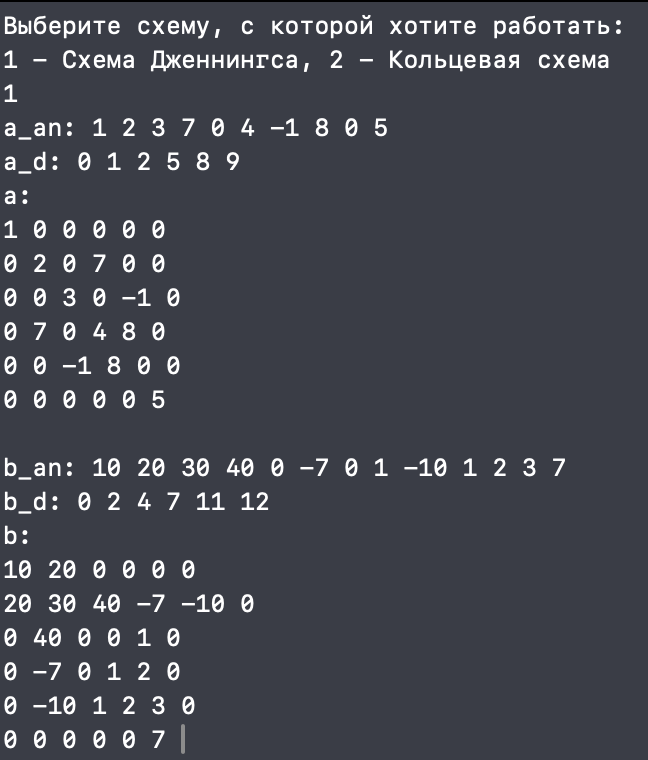
\includegraphics[scale=0.6]{Тест 1.1.png}}
 		\center{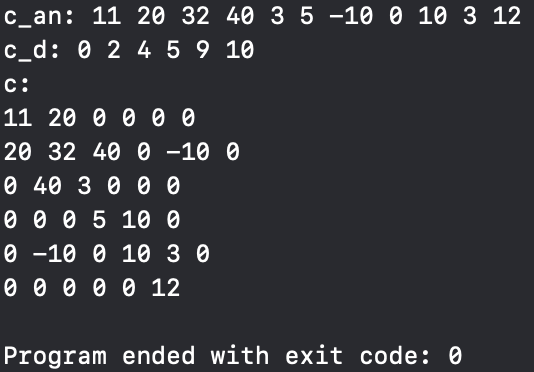
\includegraphics[scale=0.7]{Тест 1.2.png}}
  		\caption{Вывод теста 1}
	\end{figure}
	\newpage
	\item Тест 2: Входные файлы: test2.1.txt, 
	test2.2.txt --- две нулевые матрицы\\
	Вывод программы --- их нулевая сумма:
	\begin{figure}[h]
  		\center{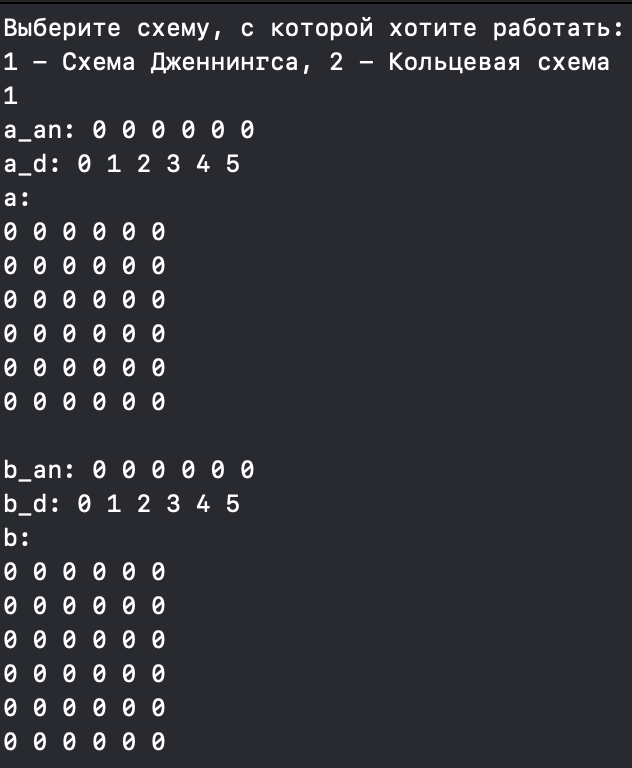
\includegraphics[scale=0.6]{Тест 2.1.png}}
 		\center{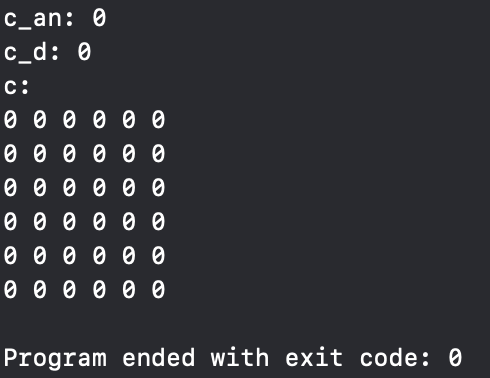
\includegraphics[scale=0.7]{Тест 2.2.png}}
  		\caption{Вывод теста 2}
	\end{figure}
	\newpage
	\item Тест 3: Входные файлы: test2.1.txt, 
	matrix2.txt --- нулевая матрица А и ненулевая матрица 
	В\\
	Вывод программы --- их сумма, то есть ненулевая матрица B:
	\begin{figure}[h]
  		\center{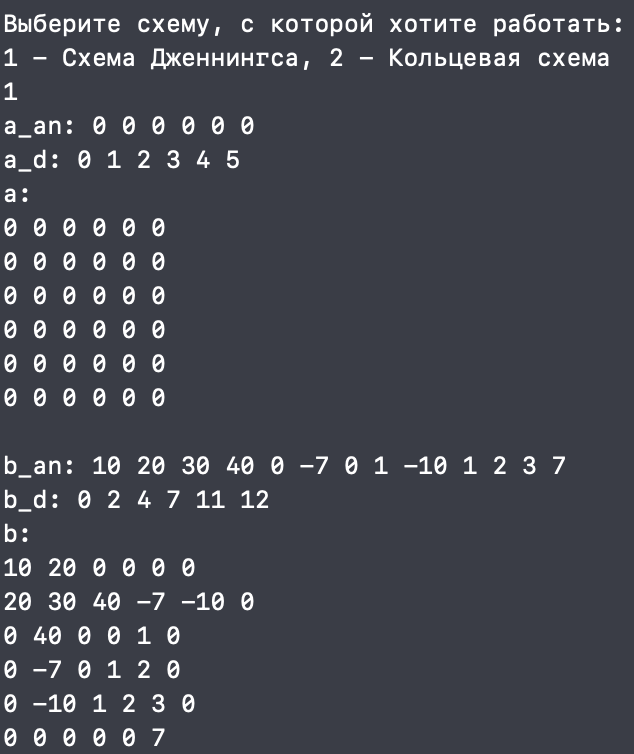
\includegraphics[scale=0.6]{Тест 3.1.png}}
 		\center{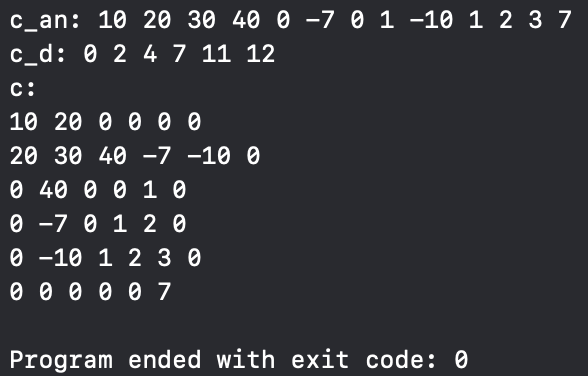
\includegraphics[scale=0.7]{Тест 3.2.png}}
  		\caption{Вывод теста 3}
	\end{figure}
	\newpage
	\item Тест 4: Входные файлы: matrix1.txt, 
	test2.2.txt --- ненулевая матрица А и нулевая матрица 
	В\\
	Вывод программы --- их сумма, то есть ненулевая матрица B:
	\begin{figure}[h]
  		\center{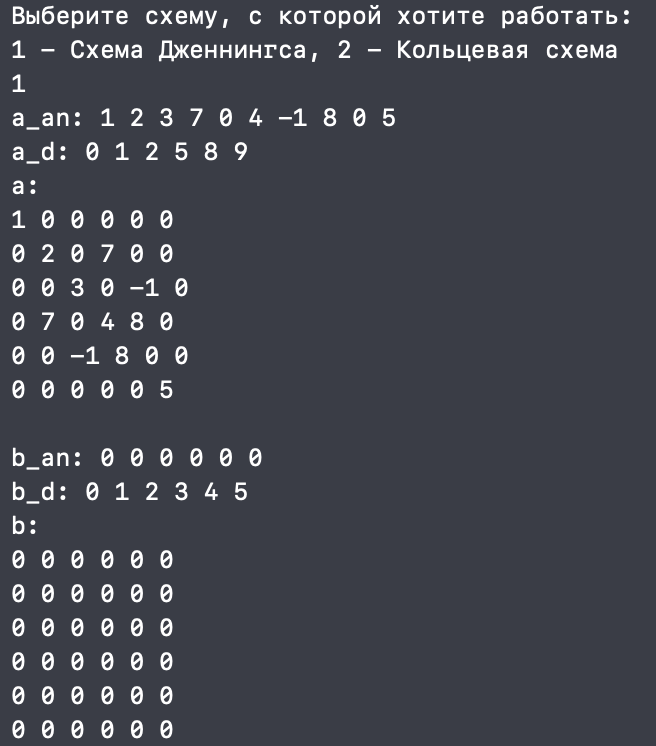
\includegraphics[scale=0.6]{Тест 4.1.png}}
 		\center{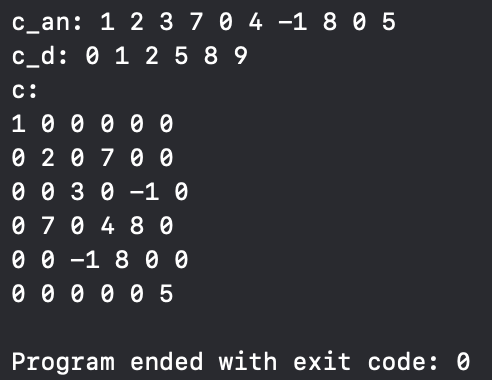
\includegraphics[scale=0.7]{Тест 4.2.png}}
  		\caption{Вывод теста 4}
	\end{figure}
	\newpage
	\item Тест 5: Входные файлы: matrix1.txt, 
	test5.txt --- матрицы, которые невозможно сложить\\
	Вывод программы --- ошибка:
	\begin{figure}[h]
  		\center{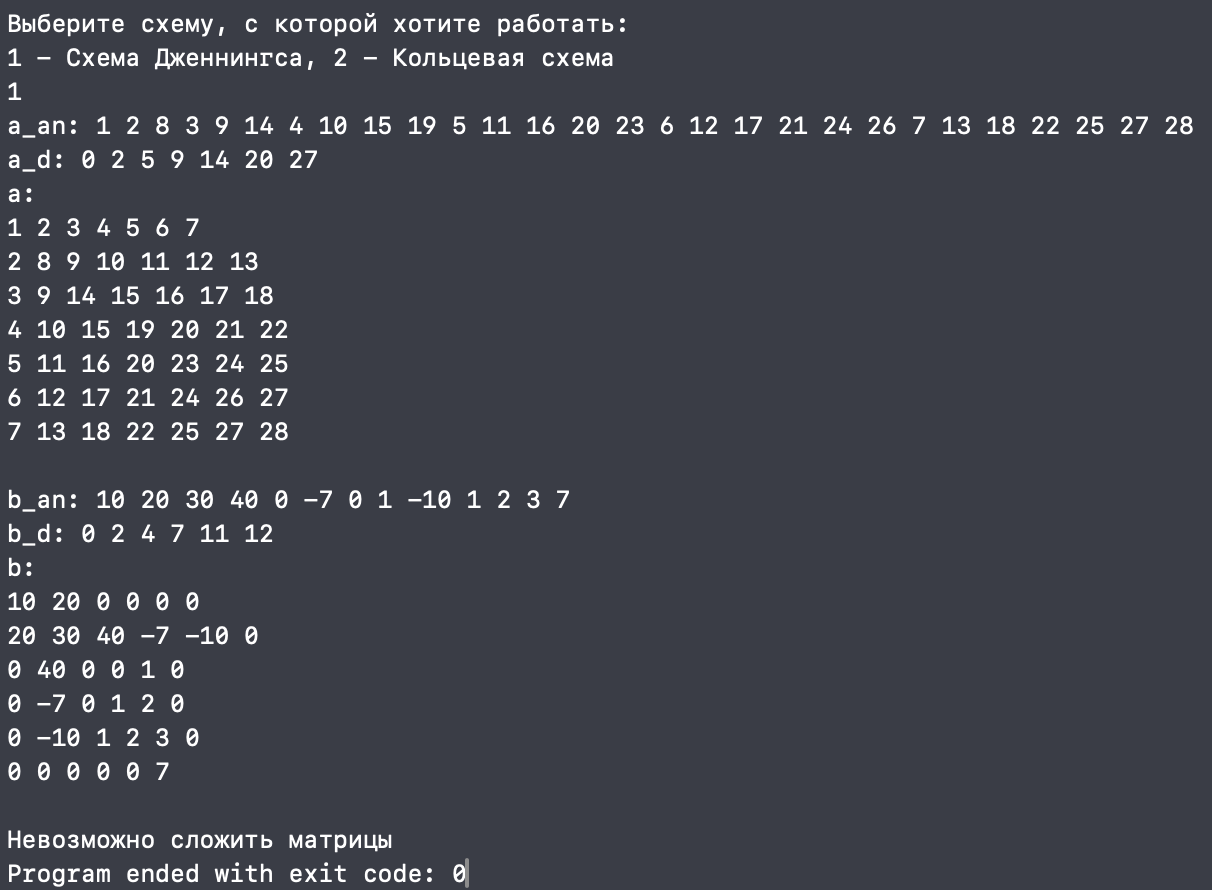
\includegraphics[scale=0.6]{Тест 5.png}}
  		\caption{Вывод теста 5}
	\end{figure}
	\newpage
	\item Тест 6: Входные файлы: test6.1.txt, 
	test6.2.txt --- матрицы 3 на 3
	Вывод программы --- сумма двух матриц 3 на 3:
	\begin{figure}[h]
  		\center{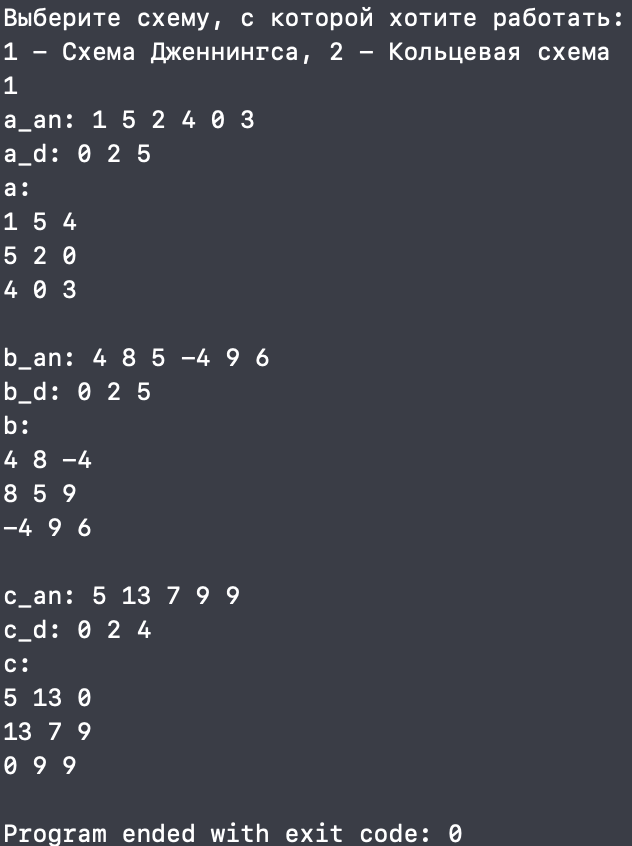
\includegraphics[scale=0.7]{Тест 6.png}}
  		\caption{Вывод теста 6}
	\end{figure}
\end{enumerate}
\newpage
\subsection{Кольцевая схема Рейнбольдта-Местеньи, сложение матриц}
Ниже приведены тесты работы программы, которая суммирует произвольные матрицы, 
упакованные по кольцевой схеме Рейнбольдта-Местеньи
\begin{enumerate}
	\item Тест 7:
	Входные файлы: matrix1.txt, 
	matrix2.txt --- две ненулевые матрицы\\
	Вывод программы --- их ненулевая сумму:
	\begin{figure}[h]
  		\center{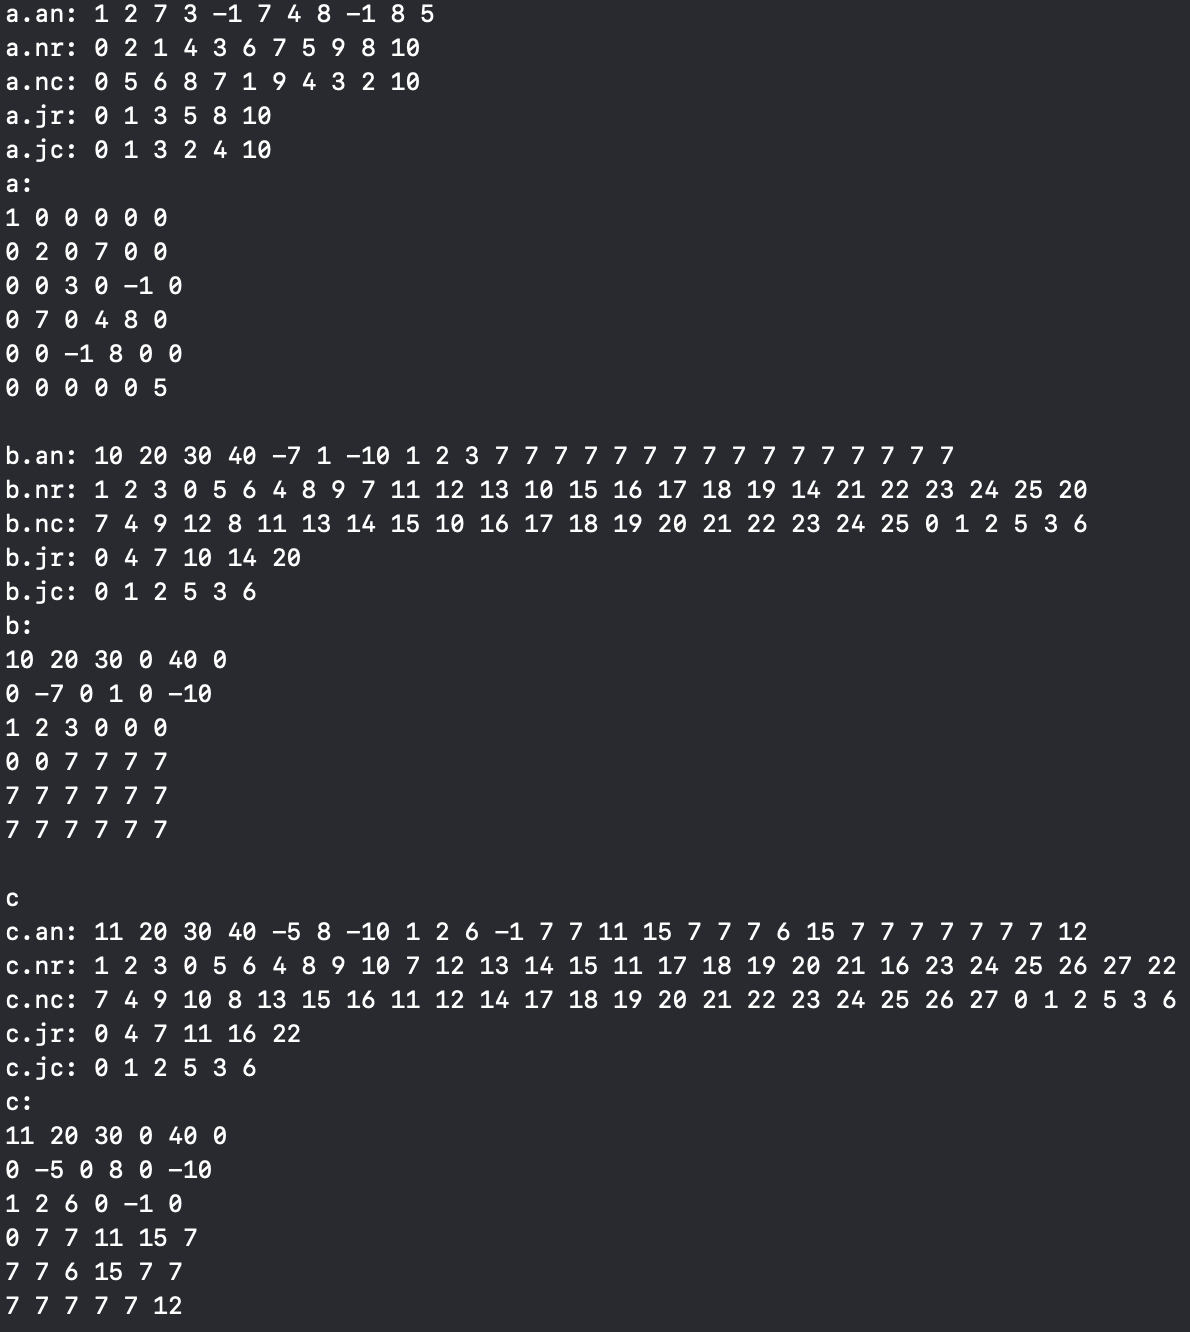
\includegraphics[scale=0.6]{Тест 7.png}}
  		\caption{Вывод теста 7}
	\end{figure}
	\newpage
	\item Тест 8: Входные файлы: test2.1.txt, 
	test2.2.txt --- две нулевые матрицы\\
	Вывод программы --- их нулевая сумма:
	\begin{figure}[h]
  		\center{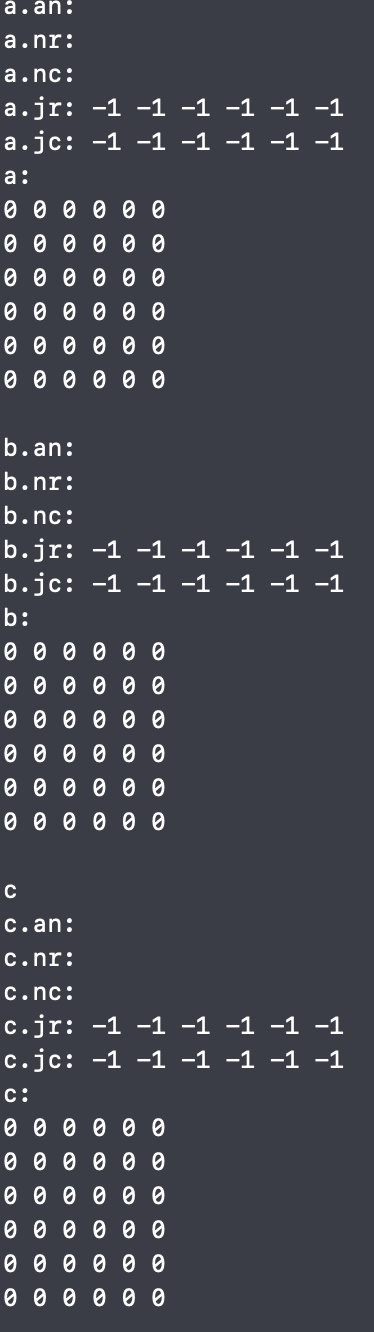
\includegraphics[scale=0.6]{Тест 8.png}}
  		\caption{Вывод теста 8}
	\end{figure}
	\newpage
	\item Тест 9: Входные файлы: test2.1.txt, 
	matrix2.txt --- нулевая матрица А и ненулевая матрица 
	В\\
	Вывод программы --- их сумма, то есть ненулевая матрица B:
	\begin{figure}[h]
  		\center{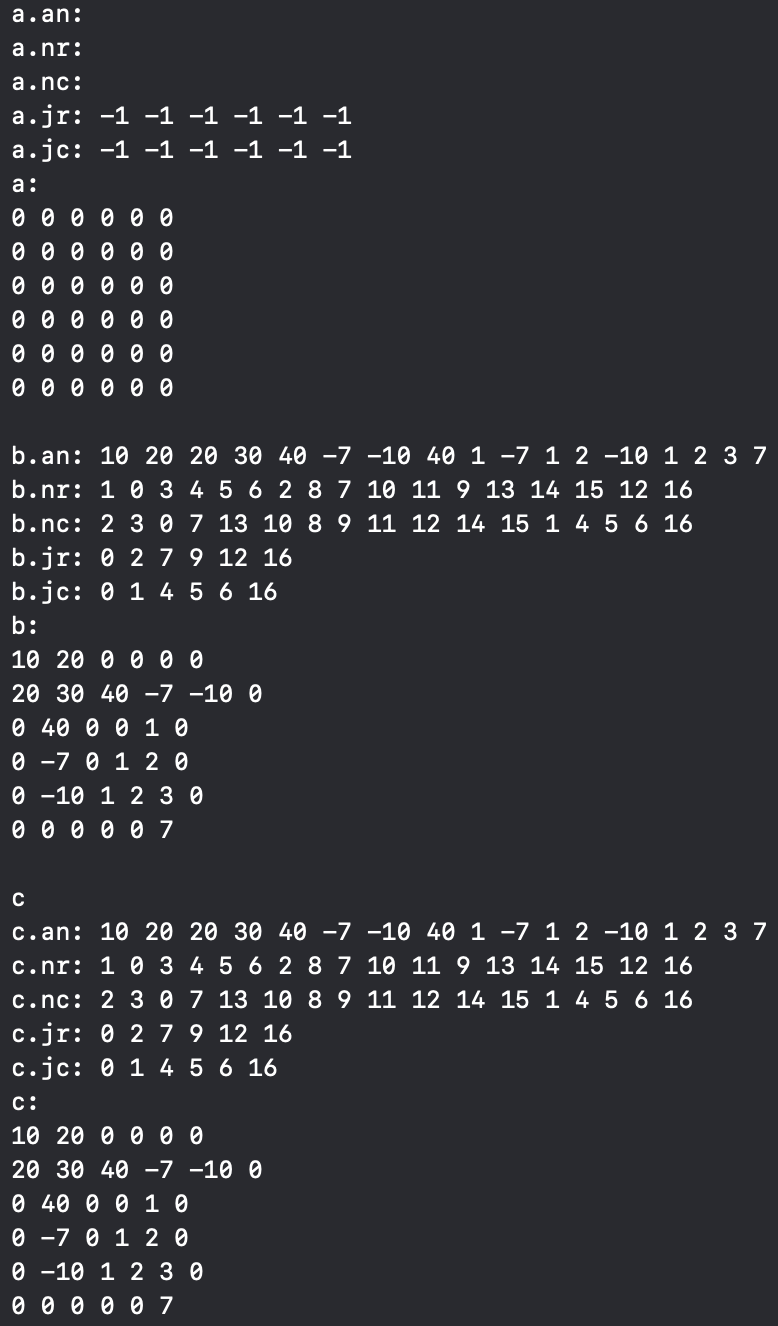
\includegraphics[scale=0.6]{Тест 9.png}}
  		\caption{Вывод теста 9}
	\end{figure}
	\newpage
	\item Тест 10: Входные файлы: matrix1.txt, 
	test2.2.txt --- ненулевая матрица А и нулевая матрица 
	В\\
	Вывод программы --- их сумма, то есть ненулевая матрица A:
	\begin{figure}[h]
  		\center{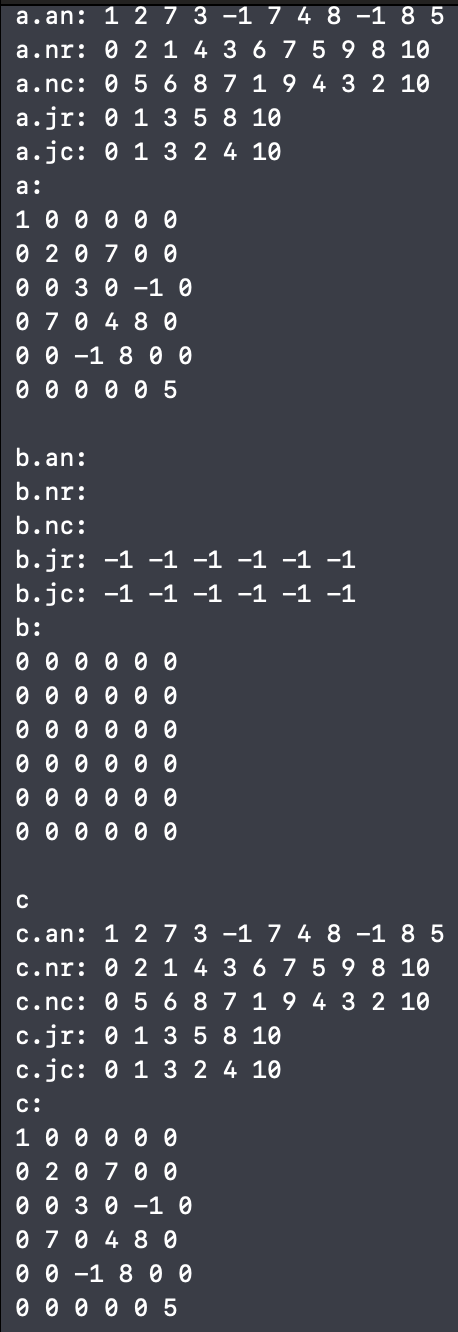
\includegraphics[scale=0.6]{Тест 10.png}}
  		\caption{Вывод теста 10}
	\end{figure}
	\newpage
	\item Тест 11: Входные файлы: matrix1.txt, 
	test5.txt --- матрицы, которые невозможно сложить\\
	Вывод программы --- ошибка:
	\begin{figure}[h]
  		\center{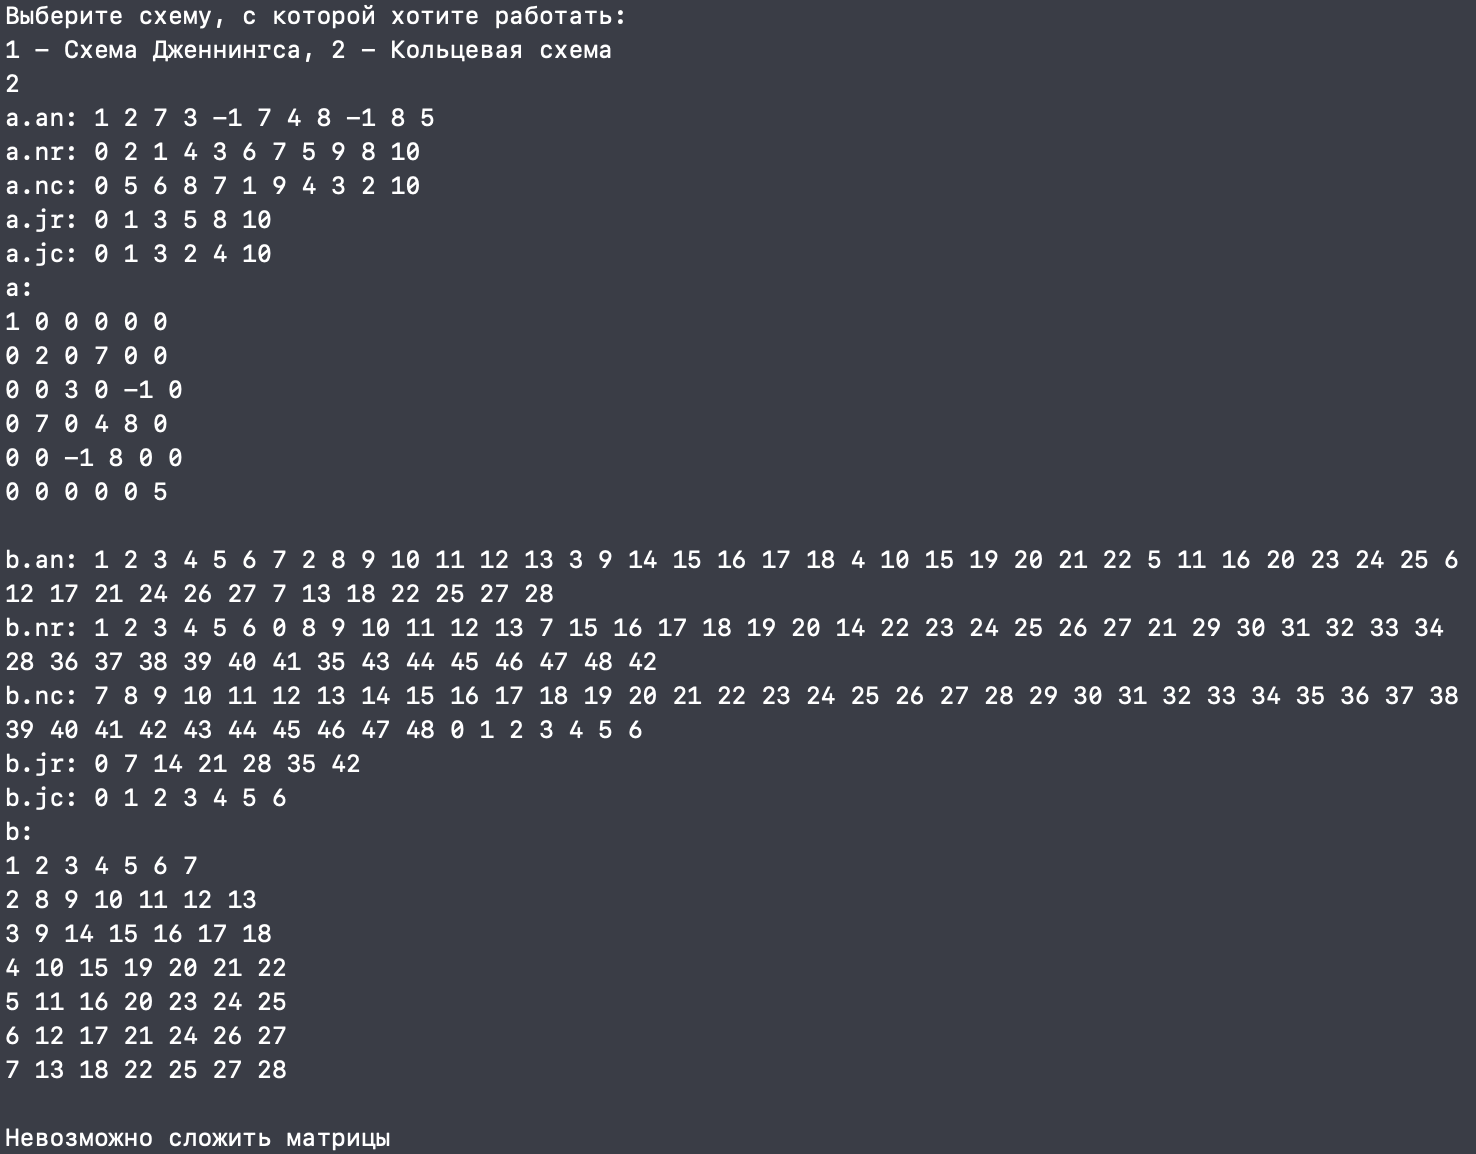
\includegraphics[scale=0.6]{Тест 11.png}}
  		\caption{Вывод теста 11}
	\end{figure}
	\newpage
	\item Тест 12: Входные файлы: test6.1.txt, 
	test6.2.txt --- матрицы 3 на 3
	Вывод программы --- сумма матриц размера 3 на 3:
	\begin{figure}[h]
  		\center{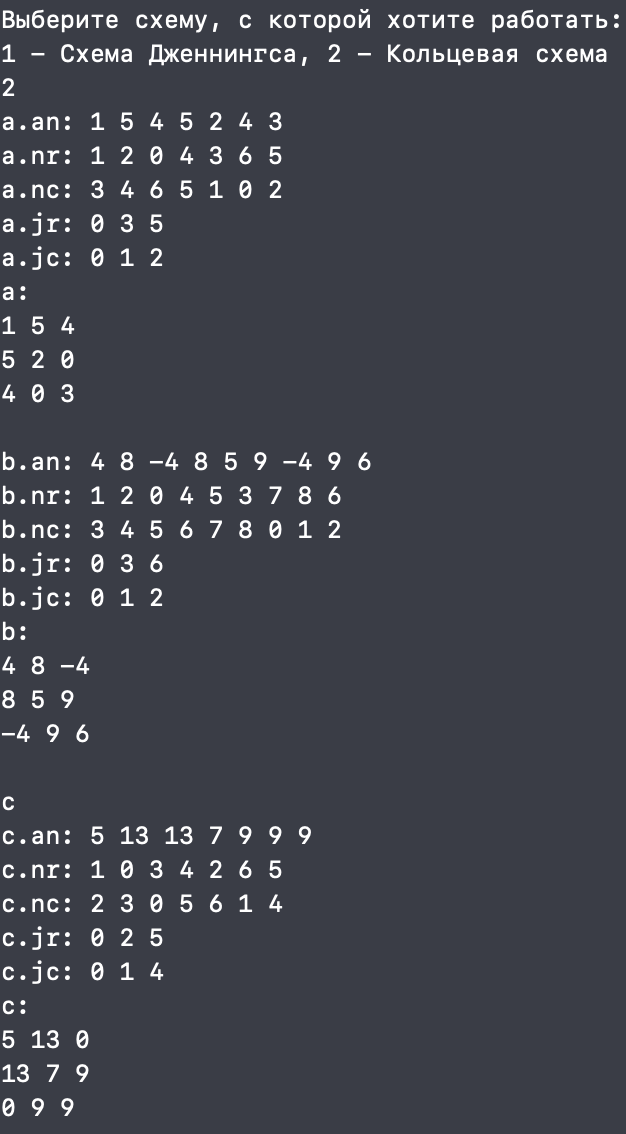
\includegraphics[scale=0.7]{Тест 12.png}}
  		\caption{Вывод теста 12}
	\end{figure}
\end{enumerate}
\newpage
\subsection{Кольцевая схема Рейнбольдта-Местеньи, умножение матриц}
Ниже приведены тесты работы программы, которая умножает произвольные матрицы, 
упакованные по кольцевой схеме Рейнбольдта-Местеньи
\begin{enumerate}
	\item Тест 13:
	Входные файлы: matrix4.txt, 
	matrix5.txt --- две ненулевые матрицы\\
	Вывод программы --- произведение двух матриц:
	\begin{figure}[h]
  		\center{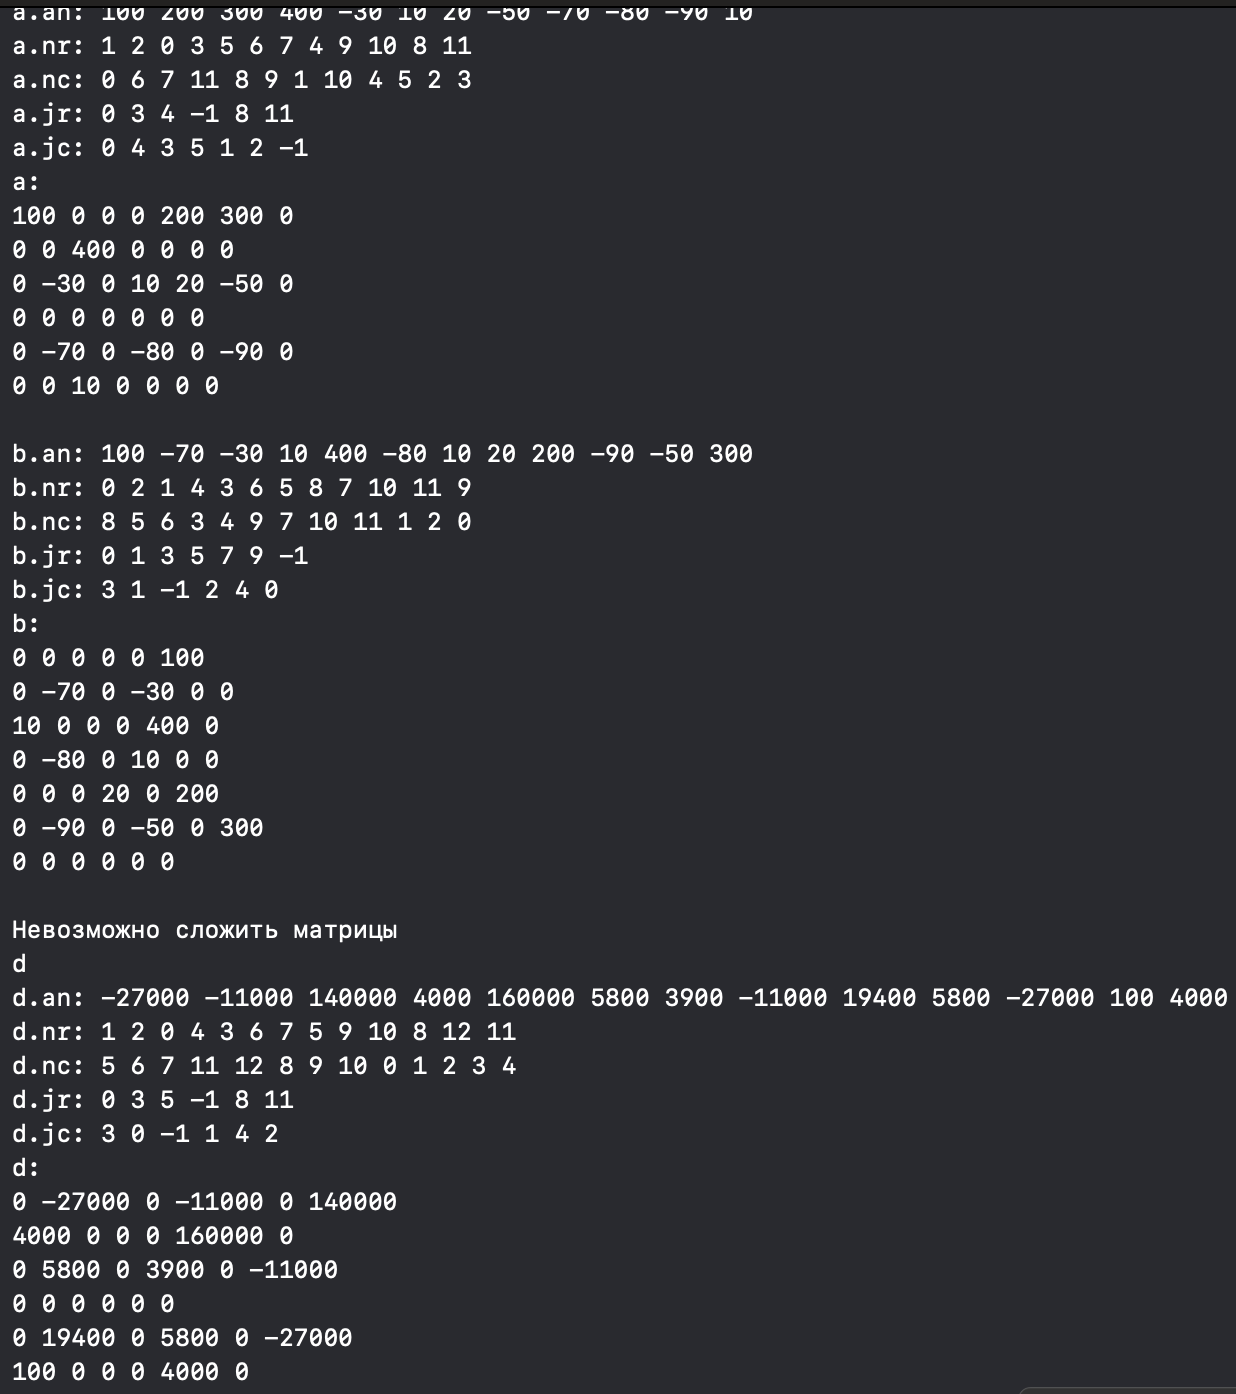
\includegraphics[scale=0.6]{Тест 13.png}}
  		\caption{Вывод теста 13}
	\end{figure}
	\newpage
	\item Тест 14: Входные файлы: test14.1.txt, 
	test14.2.txt --- две нулевые матрицы\\
	Вывод программы --- нулевое произведение двух нулевых матриц:
	\begin{figure}[h]
  		\center{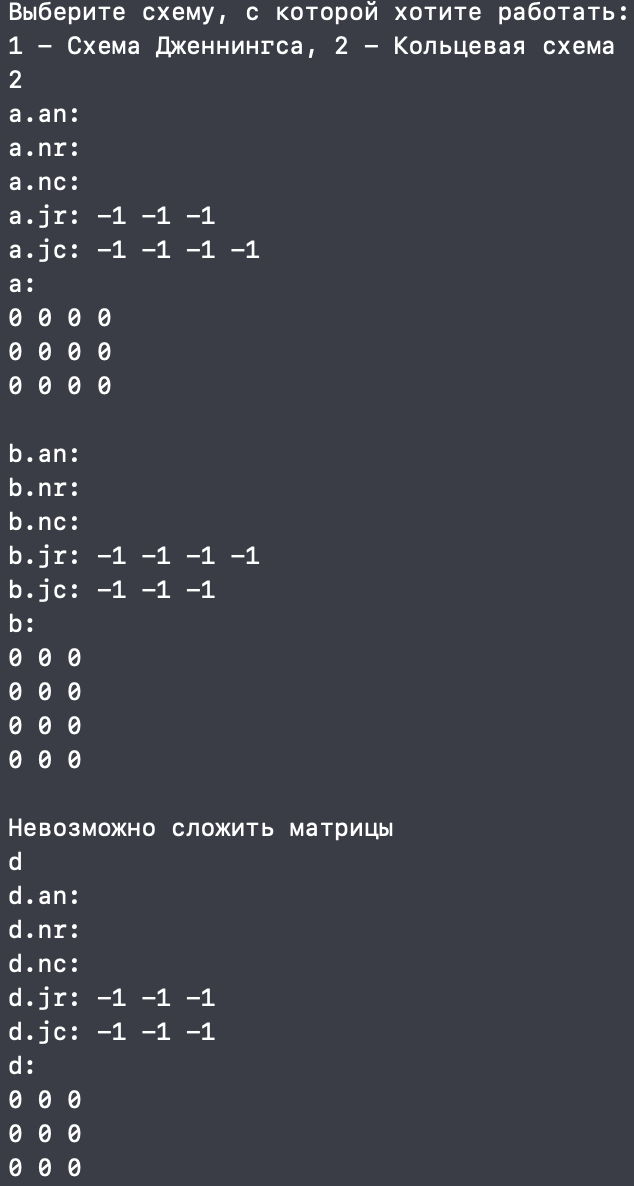
\includegraphics[scale=0.6]{Тест 14.png}}
  		\caption{Вывод теста 14}
	\end{figure}
	\newpage
	\item Тест 15: Входные файлы: test14.1.txt, 
	matrix5.txt --- нулевая матрица А и ненулевая матрица 
	В\\
	Вывод программы --- нулевое произведение одной нулевой и одной ненулевой 
	матрицы:
	\begin{figure}[h]
  		\center{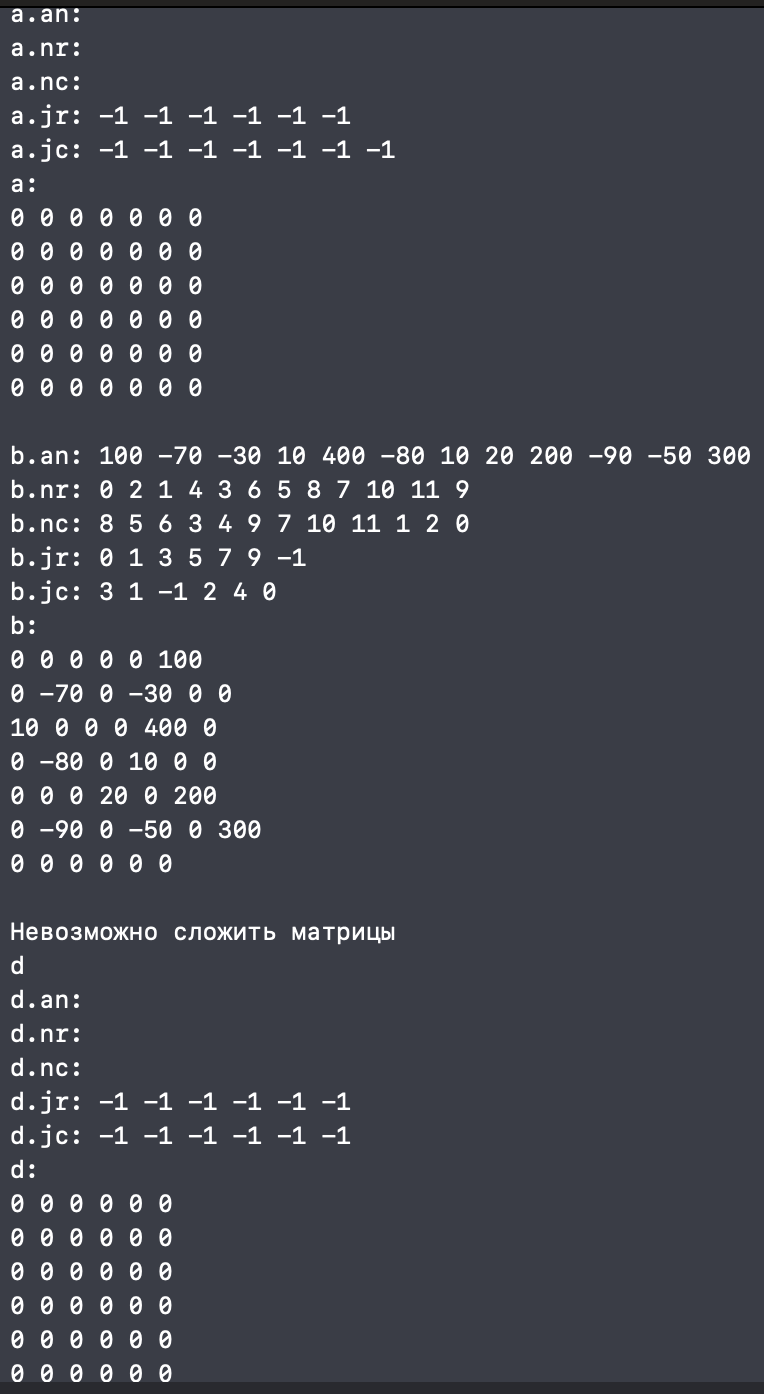
\includegraphics[scale=0.6]{Тест 15.png}}
  		\caption{Вывод теста 15}
	\end{figure}
	\newpage
	\item Тест 16: Входные файлы: matrix4.txt, 
	test14.2.txt --- ненулевая матрица А и нулевая матрица 
	В\\
	Вывод программы --- нулевое произведение одной нулевой и одной ненулевой 
	матрицы:
	\begin{figure}[h]
  		\center{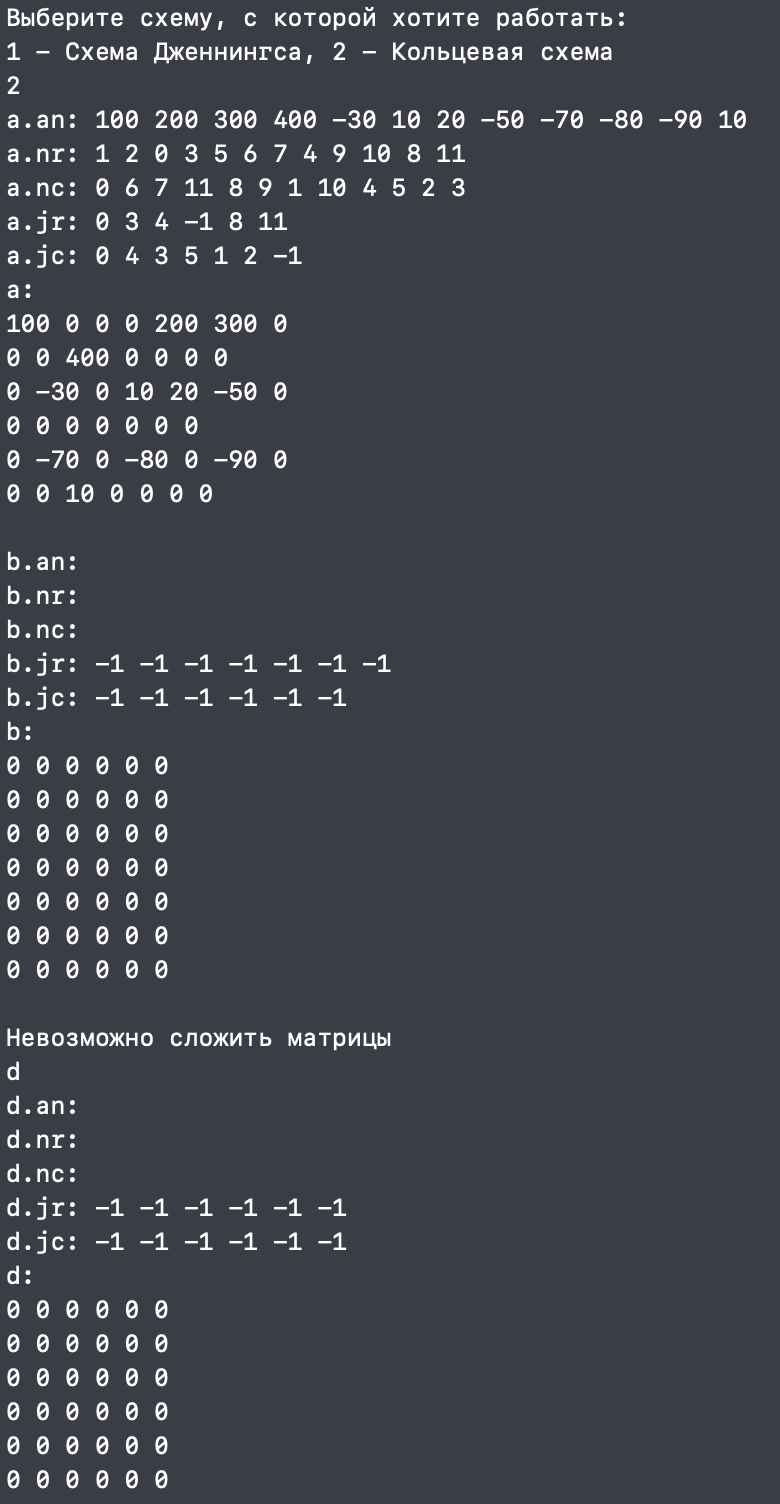
\includegraphics[scale=0.6]{Тест 16.png}}
  		\caption{Вывод теста 16}
	\end{figure}
	\newpage
	\item Тест 17: Входные файлы: matrix1.txt, 
	matrix3.txt --- матрицы, которые невозможно перемножить\\
	Вывод программы --- ошибка:
	\begin{figure}[h]
  		\center{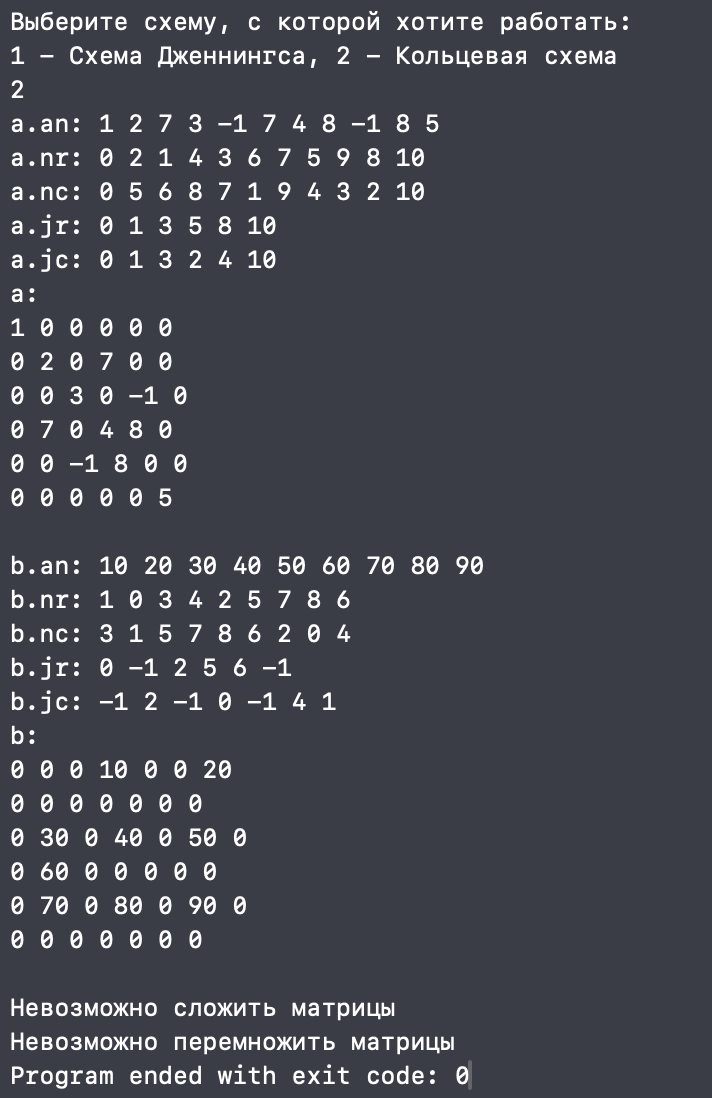
\includegraphics[scale=0.6]{Тест 17.png}}
  		\caption{Вывод теста 17}
	\end{figure}
	\newpage
	\item Тест 18: Входные файлы: test18.1.txt, 
	test18.2.txt --- матрица 3 на 2 и 2 на 3
	Вывод программы --- произведение двух матриц:
	\begin{figure}[h]
  		\center{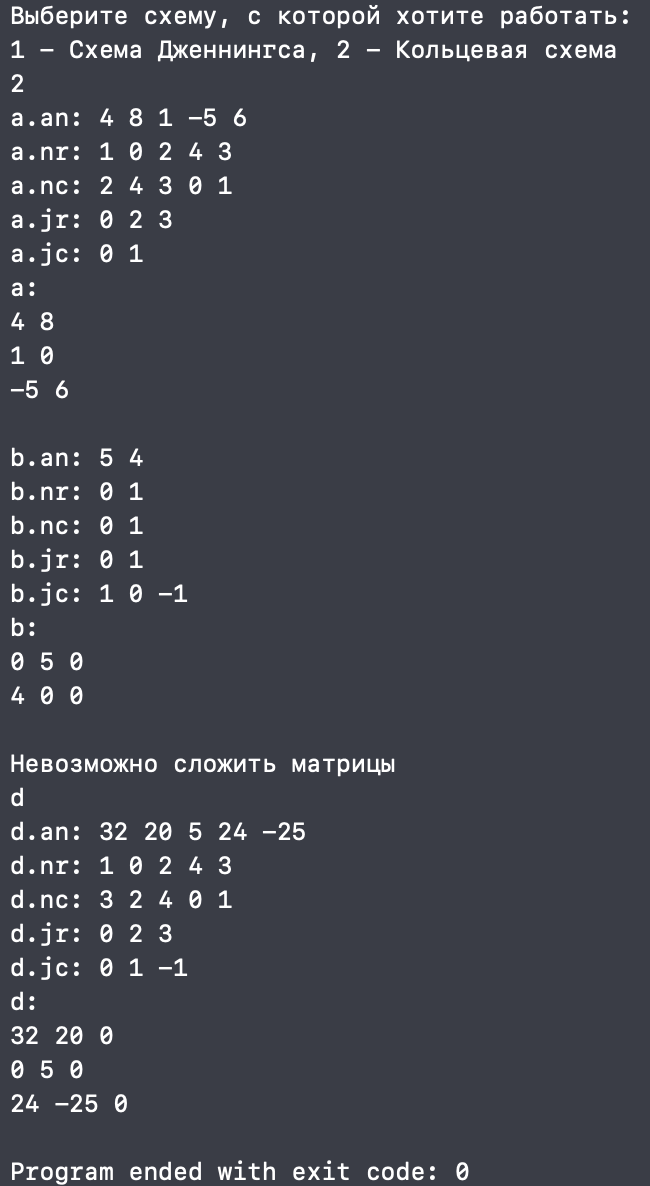
\includegraphics[scale=0.7]{Тест 18.png}}
  		\caption{Вывод теста 18}
	\end{figure}
\end{enumerate}
\newpage
\section{Примеры работы}
\subsection{Схема Дженнингса}
Ниже представлены примеры работы функций для матриц, упакованных по схеме 
Дженнингса:
\begin{enumerate}
	\item На вход подаются две произвольные матрицы, программа выводит их сумму
	\begin{figure}[h]
  		\center{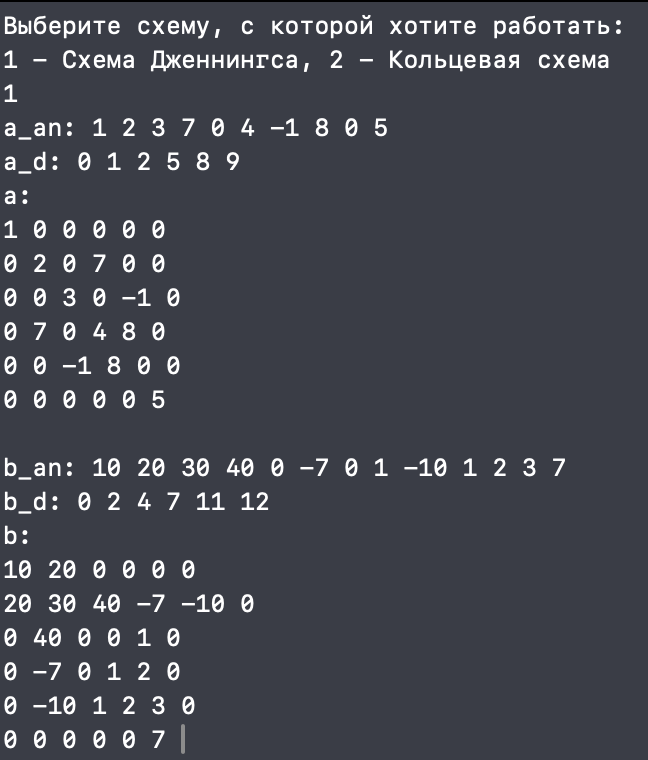
\includegraphics[scale=0.6]{Тест 1.1.png}}
 		\center{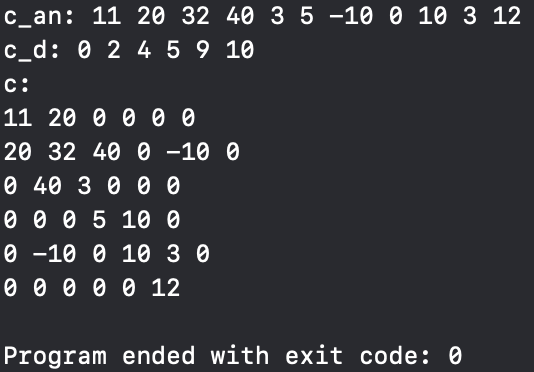
\includegraphics[scale=0.7]{Тест 1.2.png}}
  		\caption{Пример работы 1}
	\end{figure}
	\newpage
	\item На вход подаются матрицы разных размерностей, которые невозможно 
	сложить, программа выдает ошибку
	\begin{figure}[h]
  		\center{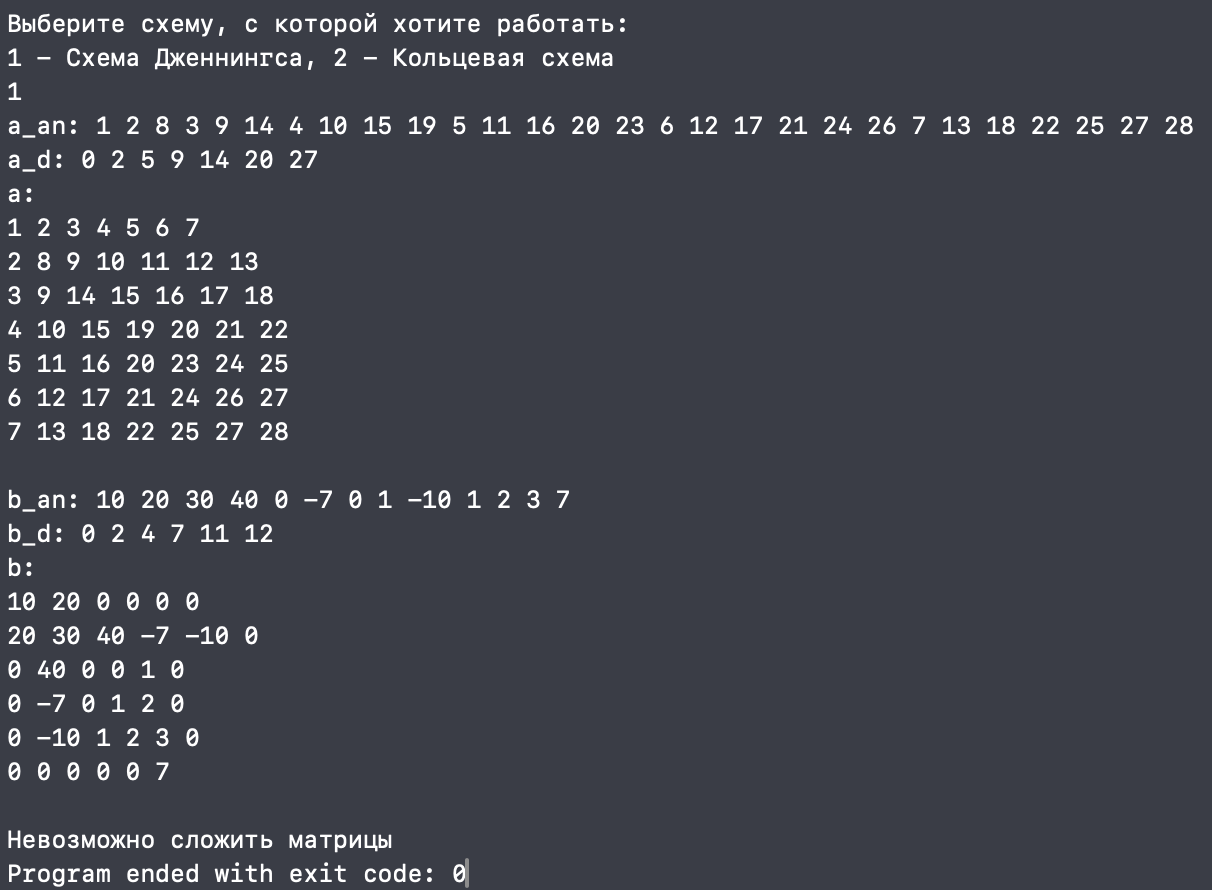
\includegraphics[scale=0.6]{Тест 5.png}}
  		\caption{Пример работы 2}
	\end{figure}
\newpage
\end{enumerate}
\subsection{Кольцевая схема Рейнбольдта-Местеньи}
Ниже представлены примеры работы функций для матриц, упакованных по схеме 
кольцевой схема Рейнбольдта-Местеньи
\begin{enumerate}
	\item На вход подаются две произвольные матрицы, программа выводит их 
	произведение	
	\begin{figure}[h]
  		\center{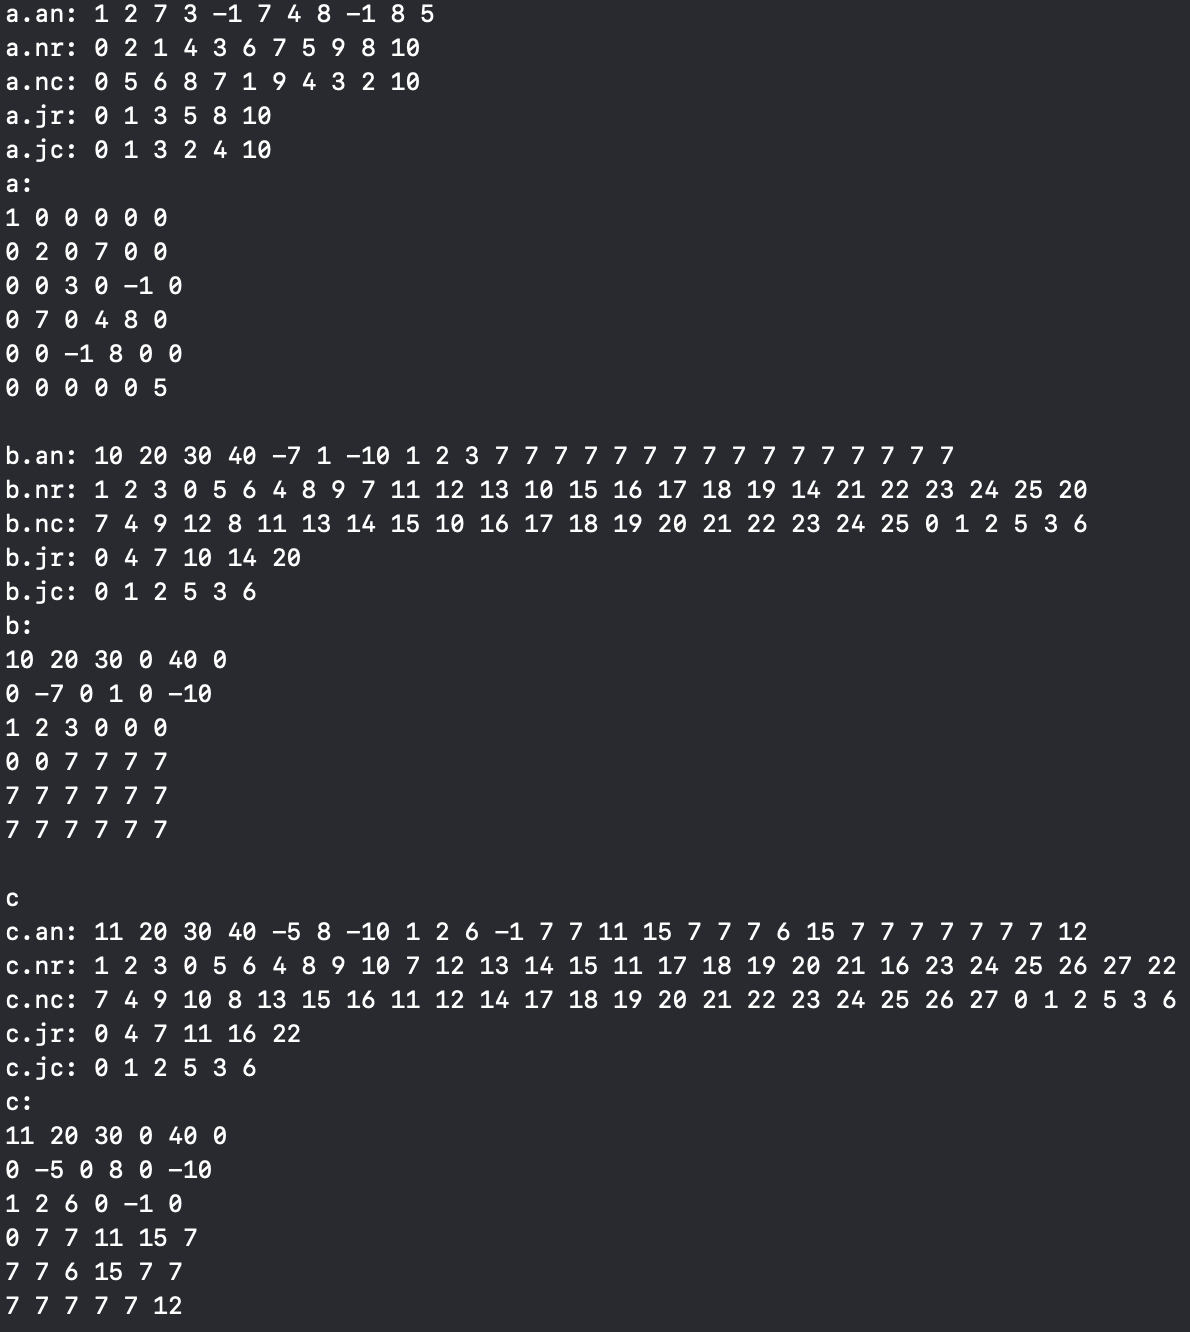
\includegraphics[scale=0.6]{Тест 7.png}}
  		\caption{Пример работы 3}
	\end{figure}
	\newpage
	\item На вход подаются матрицы разных размерностей, которые невозможно 
	сложить, программа выдает ошибку
	\begin{figure}[h]
  		\center{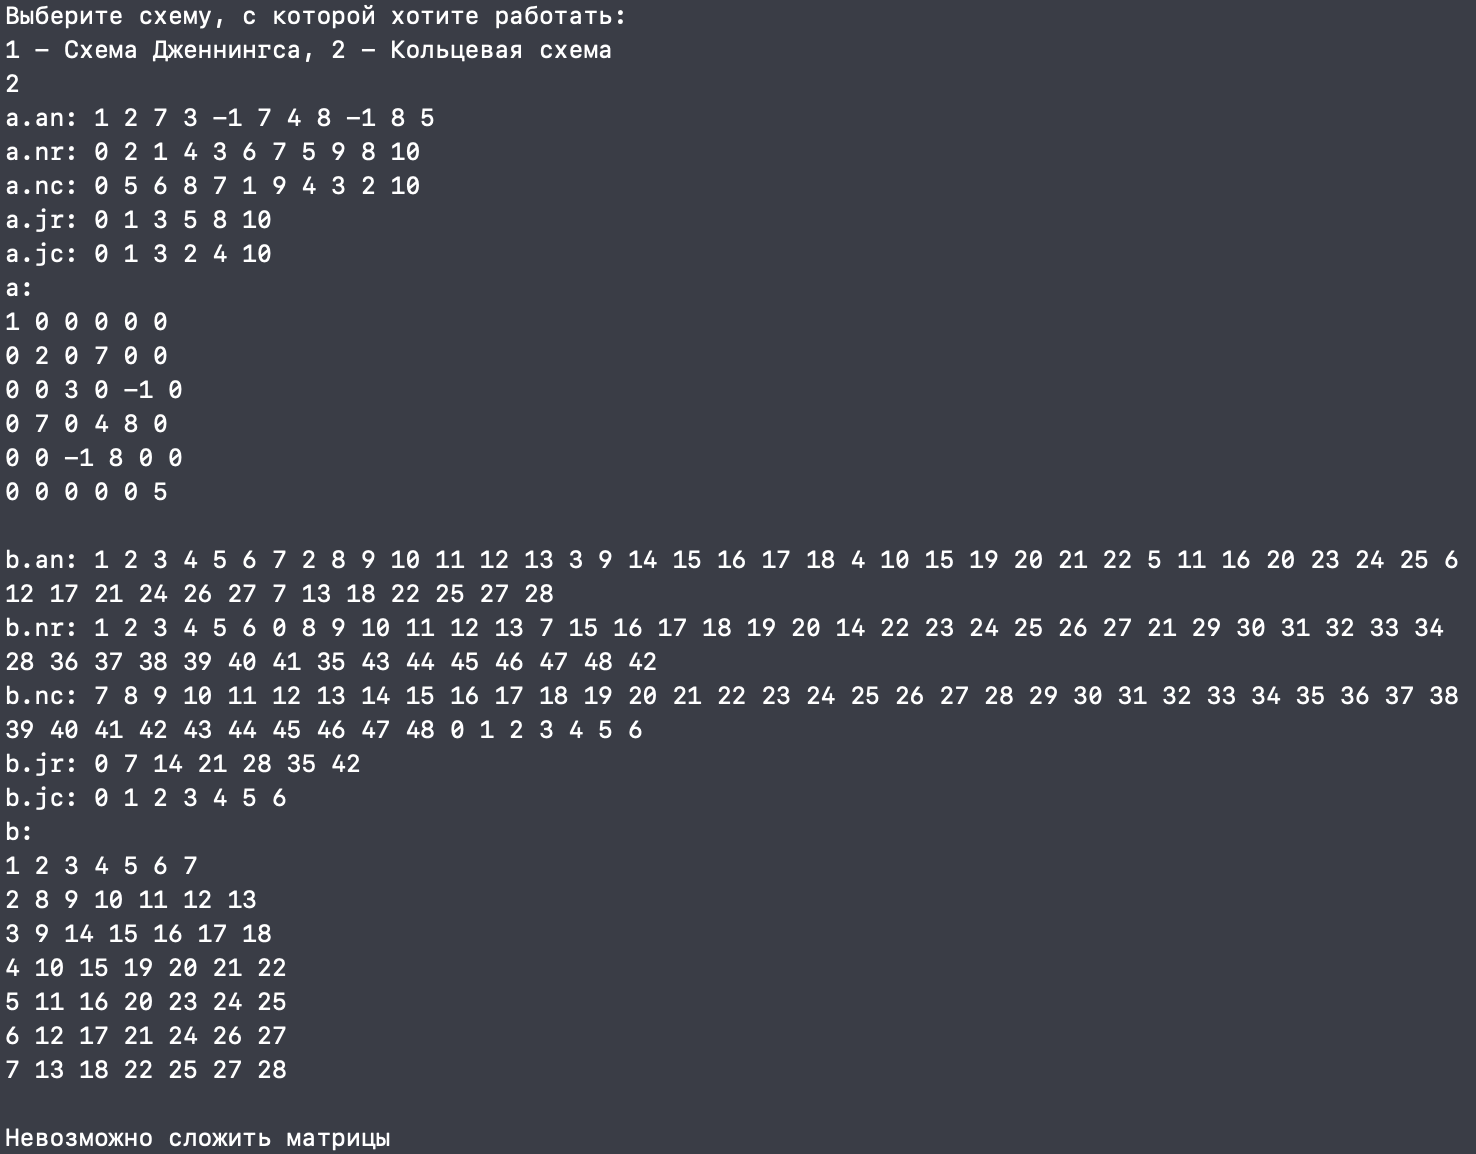
\includegraphics[scale=0.6]{Тест 11.png}}
  		\caption{Пример работы 3}
	\end{figure}
	\newpage
	\item На вход подаются две произвольные матрицы, программа выводит их сумму	
	\begin{figure}[h]
  		\center{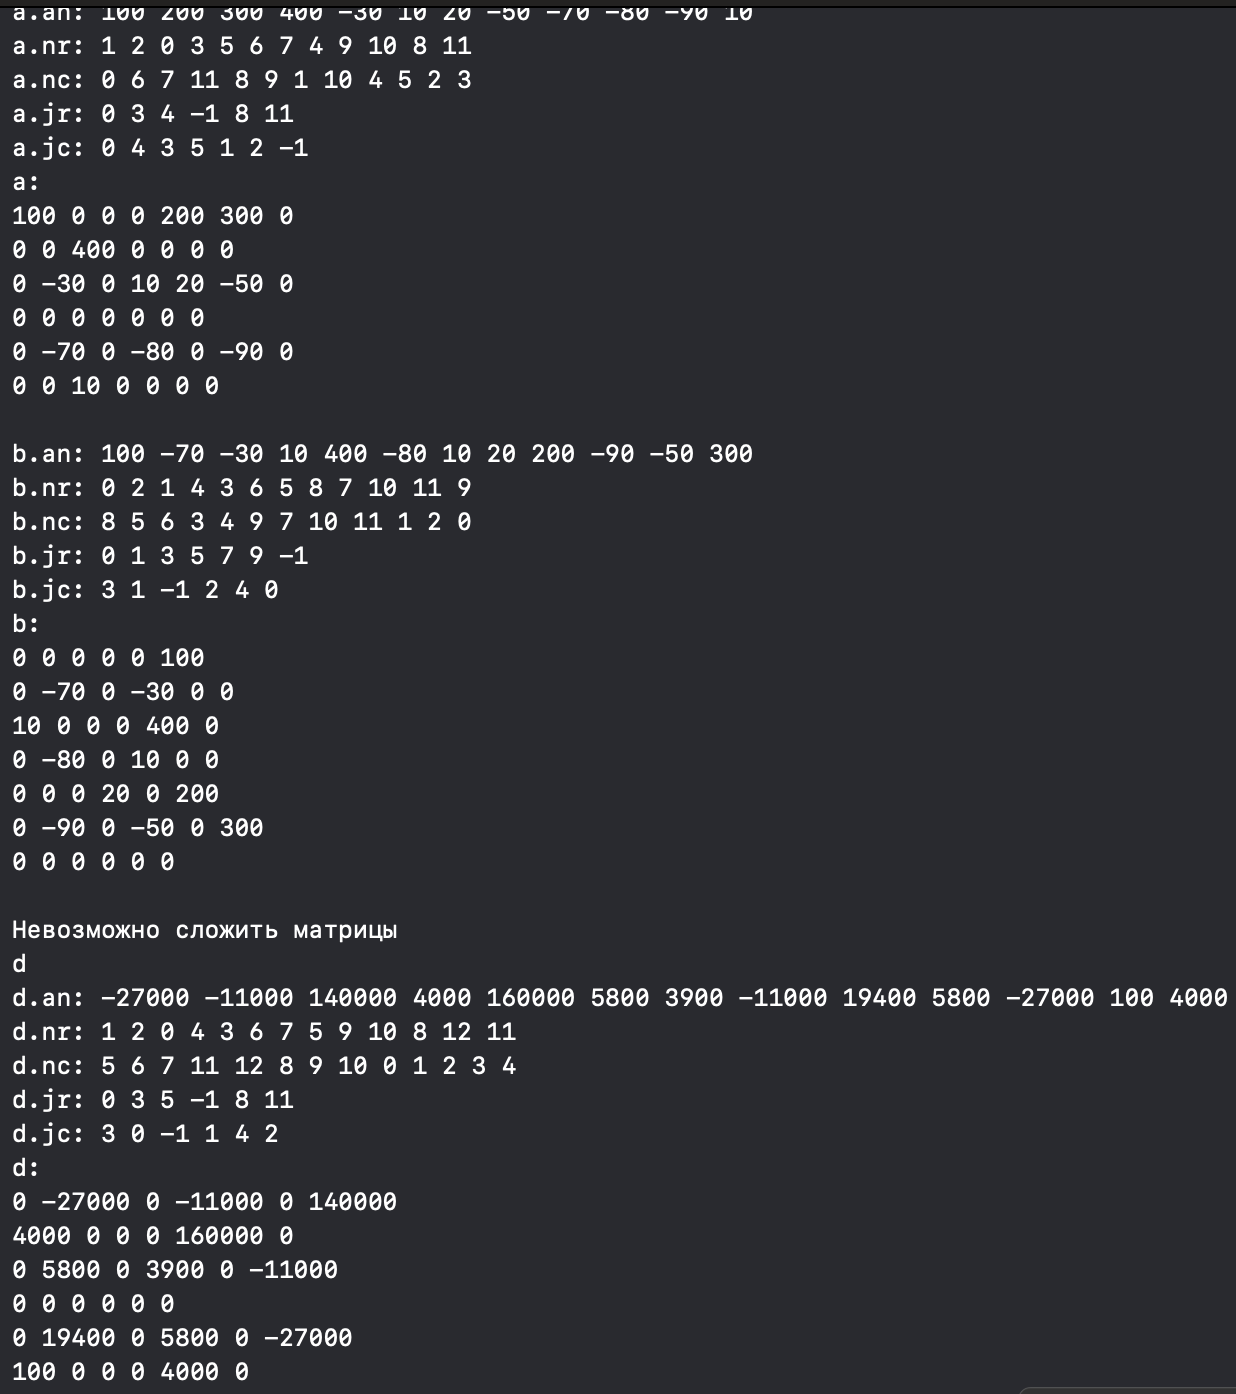
\includegraphics[scale=0.6]{Тест 13.png}}
  		\caption{Пример работы 4}
	\end{figure}
	\newpage
	\item На вход подаются матрицы, которые невозможно 
	умножить, программа выдает ошибку
	\begin{figure}[h]
  		\center{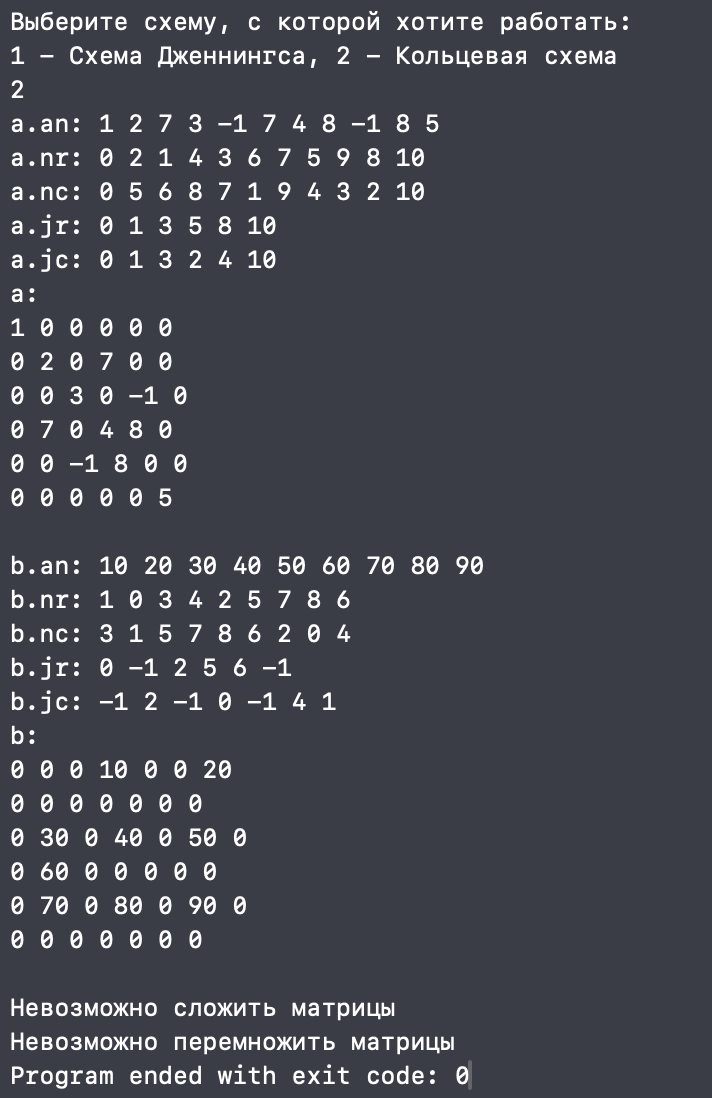
\includegraphics[scale=0.6]{Тест 17.png}}
  		\caption{Пример работы 4}
	\end{figure}
\end{enumerate}
\newpage
\section{Заключение}
Цель достигнута: 
\begin{enumerate}
\item Рассмотрены две схемы хранения матриц и реализованы функции:
\begin{enumerate}
	\item $show\_one\_dim$ --- вывод на экран одномерный 
	вектор;
	\item $show\_two\_dim$ --- вывод на экран двумерный
	вектор;
	\item $comp\_Djen$ --- упаковка матрицы по схеме
	Дженнингса;
	\item $sum\_Djen$ --- сумма двух матриц, упакованных 
	по схеме Дженнингса;
	\item $unpack\_Djen$ --- распаковка матрицы, 
	упакованной по схеме Дженнингса.
	\item $add\_element$ --- добавления элемента в упакованную по кольцевой 
	схеме матрицу;
	\item $comp\_ring\_RM$ --- упаковка матрицы по 
	кольцевой схеме;
	\item $col\_el$ --- поиск столбцовой координаты
	элемента;
	\item $row\_el$ --- поиск строчной координаты
	элемента;
	\item $unpack\_ring\_RM$ --- распаковка матрицы, 
	упакованной по кольцевой схеме;
	\item $sum\_ring\_RM$ --- сумма двух матриц, 
	упакованных по кольцевой схеме;
	\item $mult\_ring\_RM$ --- произведение двух матриц, 
	упакованных по кольцевой схеме.
\end{enumerate}
\item Выполнено тестирование реализации разработанных функций.
\item Проведен анализ эффективности сжатого хранения матриц в обоих схемах для 
матрицы действительных чисел с 5~\% ненулевых элементов.
\end{enumerate}
\newpage
\begin{center}
\begin{thebibliography}{}
\addcontentsline{toc}{section}{Список используемых источников}
\bibitem{book}Писсанецки, С. Технология разреженных матриц [Текст]: монография / С.Писсанецки.; пер. с анг. под ред. Х.Д.Икрамова. - М.: Мир, 1988. - 410 с.
\end{thebibliography}
\end{center}
\end{document}
